%!TEX root = thesis.tex
\chapter{Active nematics on the surface of a torus}\label{c:3}
\section{Introduction}
Active materials are composed of constituent particles that each can convert stored internal energy or ambient energy to kinetic energy, thus driving the material out-of equilibrium~\cite{RN237,RN238,RN40}.
Importantly, this is distinct from global driving mechanisms such as the application of a shear or the imposition of a field; in active materials, the material is driven out-of-equilibrium due to the intrinsic nonequilibrium behavior of the constituent particles.
Thus, the material cannot be understood within the framework of equilibrium statistical mechanics as the individual particles are subject to forces independent of those provided by thermal fluctuations.
However, this also means that active materials can be composed of constituents of any size, as activity does not care if the constituent particles are thermal or athermal.
For example, the framework of ``active matter'' has been used to study self-organization and self-driven behavior in flocks of starlings~\cite{RN239,RN240}, collections of robots~\cite{RN241}, colonies of fire ants~\cite{RN242}, cell growth and migration~\cite{RN51,RN160}, and self-propelled colloidal particles~\cite{RN168,RN38}.
Note that these examples of active matter span 6 orders of magnitude in size, from the starlings at $\mathcal{O}(10^-1)$ m to the colloidal particles at $\mathcal{O}(10^-7)$ m, with behavior such as flocking, giant number fluctuations, chaotic flows, and low-Reynolds number turbulence driven entirely by a single control parameter~\cite{RN237,RN238,RN40}. \\
\begin{figure}[h]
  \centering
  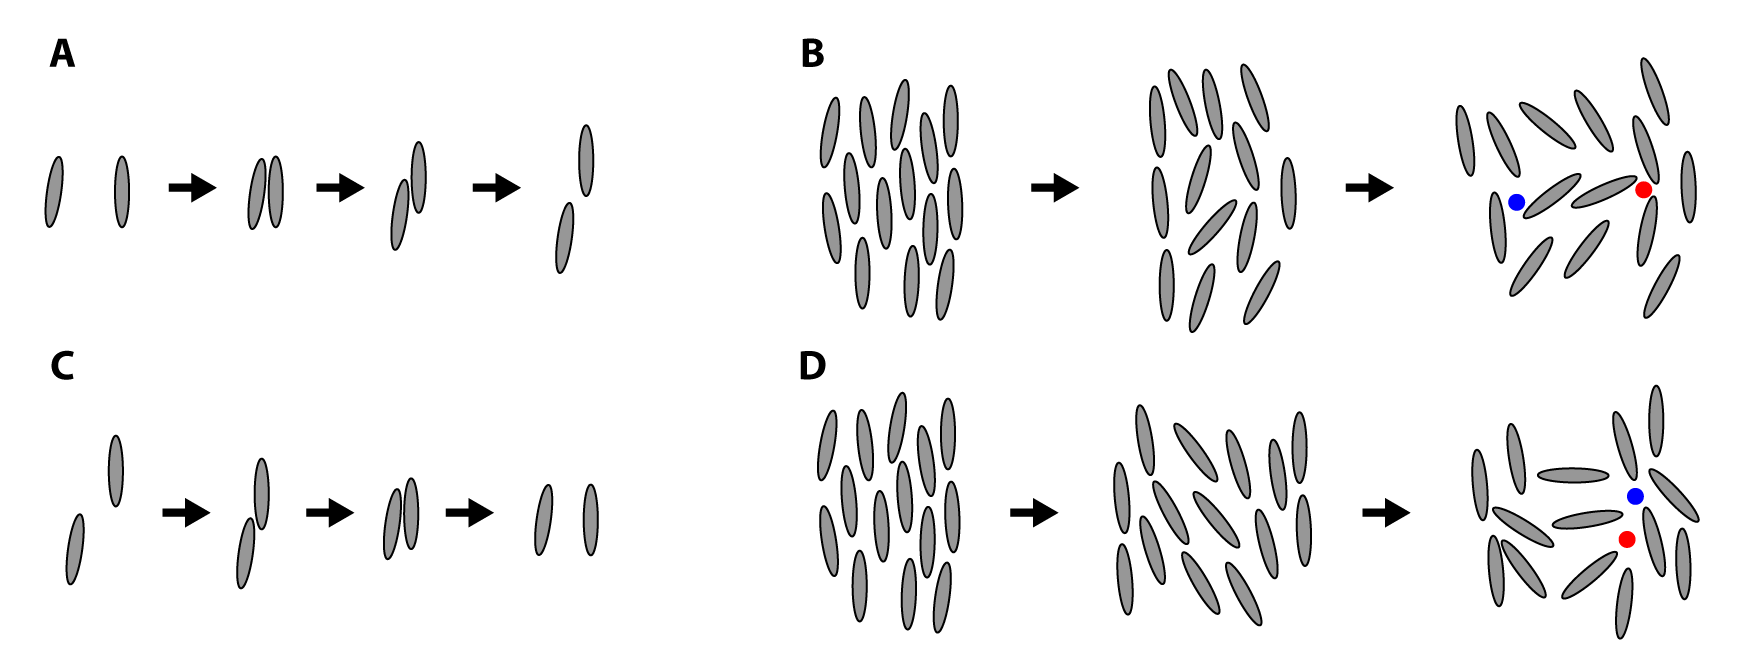
\includegraphics{figures/C3/Ch3-Figs_ActiveInteraction.png}
  \caption{Interactions in extensile and contractile nematics.
  (A,C), Two-particle interaction for extensile (A) and contractile (C) mesogens.
  The arrows represent time.
  (B,D), The homogeneous state is unstable to distortions, with (B) extensile nematics unstable to bend and (D) contractile nematics unstable to splay.
  The instability leads to the formation of an $s = + 1/2$ and $s = -1/2$ defect pair, indicated by ${\color{red} \bullet}$,${\color{blue} \bullet}$, respectively.}\label{f:3-ActiveInteraction}
\end{figure}

Much like equilibrium nematics, the individual mesogens of active nematic materials are anisotropic and thus the material possesses a nematic phase; however, the addition of activity to nematic order modifies the interaction between the mesogens.
With the exception of bacteria introduced into lyotropic liquid crystals~\cite{RN86}, to date the majority of experimental and theoretical work on active nematics takes place in 2D.
Thus, we will highlight the effect of activity on a nematic in 2D.
Consider a pair of active rod-like particles in 2D.
If the active nematic is ``extensile,'' the rods slide past each other; however, if the active nematic is ``contractile,'' the activity drives the rods to slide towards each other, as illustrated in Figure~\ref{f:3-ActiveInteraction}(A,C), respectively.
These interactions result in extensile active nematics being unstable to bend distortions while contractile active nematics are unstable to splay distortions~\cite{RN171,RN170,RN11}, as illustrated in Figure~\ref{f:3-ActiveInteraction}(B,D) respectively.
Thus, the splay and bend instabilities make the homogeneously-aligned director state unstable such that the steady-state of an active nematic is often turbulent~\cite{RN7} and full of pairs of $s = \pm 1/2$ defects that are continuously created and annihilated~\cite{RN11,RN8,RN3,RN27,RN135,RN86}.
These turbulent dynamics are driven by the $s = +1/2$ defects, where the activity coupled with the polar structure of the $s = +1/2$ defects causes the  $s = +1/2$ defects to act like self-propelled particles, with the propulsion direction depending on the type of activity~\cite{RN11,RN8}, as illustrated schematically in Figure~\ref{f:3-DefectFlow}(A).
In contrast, as shown in Figure~\ref{f:3-DefectFlow}(B), due to the three-fold symmetry of $s = -1/2$ defects, $s = -1/2$ defects are not driven by activity and are only advected by interactions between the defects as well as by interactions with the surface.\\
\begin{figure}[h]
  \centering
  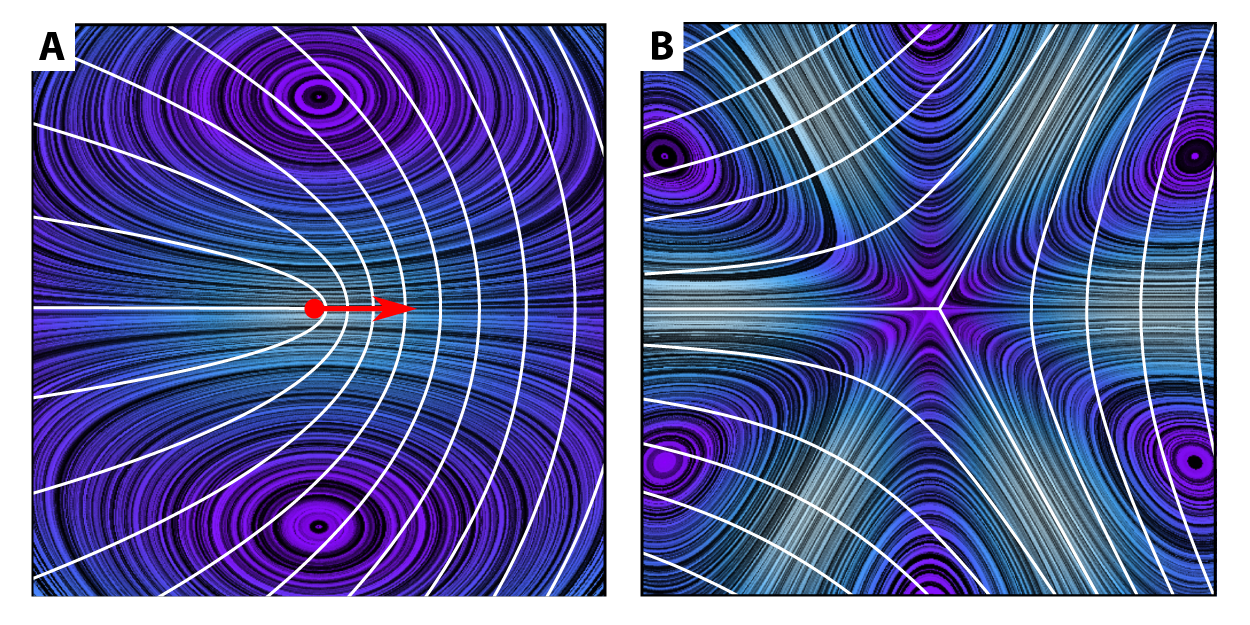
\includegraphics{figures/C3/Ch3-Figs_DefectFlow.png}
  \caption{Flow fields for active disclinations.
  (A,B) Flows generated by active (A) and $s=+1/2$ and (B) $s=-1/2$ disclinations, with the director lines drawn in white.
  Due to the polar structure of the active flow, $s = +1/2$ disclinations propel along their symmetry axis.
  The red arrow represents the propulsion direction for an extensile nematic; $s = +1/2$ disclinations will propel in the opposite direction for a contractile nematic.}\label{f:3-DefectFlow}
\end{figure}

Recent experimental studies with active nematics yielding self-regulated behaviors such as self-sustained oscillations~\cite{RN9}, spontaneous formation of morphological features such as kinks and protrusions~\cite{RN9,RN3}, and undirected motility~\cite{RN9,RN3} have acted as as stimulus to investigate how biological functionality emerges from the interplay between activity, the geometry of the system, and the structure of the internal phase~\cite{RN160,RN51,RN10}.
In this context, defects in active nematics could be harnessed to achieve life-like functionality, as defects are extremely sensitive to the intrinsic geometry of the space they inhabit.
As highlighted in Chapter~\ref{c:1}, this connection between the topological charge and the topology of the surface is easily seen in the Poincr\'e-Hopf Theorem.
However, the theory of defects in curved spaces extends this connection beyond topology, predicting that the free-energy of a collection of defects on a surface $\partial A$ is sensitive to the local geometry through the Gaussian curvature~\cite{RN42}:
\begin{equation}
  \delta F = -\frac{1}{2}\,k_{F, 2D}\int_{\partial A} \textrm{d}^2\mathbf{r}\,\textrm{d}^2\mathbf{r}'\, G(\mathbf{r},\mathbf{r}') \left[\rho(\mathbf{r})-K(\mathbf{r})] [\rho(\mathbf{r}')-K(\mathbf{r}')\right],\label{e:3-DefectsCurvedSurf}
\end{equation}
where $k_{F, 2D}$ is the Frank constant in 2D, $\rho(\mathbf{r})$ is the position-dependent defect density, and $G(\mathbf{r},\mathbf{r}')$ is the Laplacian Green's function on the surface.
Thus, similar to how the Poincar\'e-Hopf Theorem requires the total toplogical charge to be equivalent to the integrated Gaussian curvature, Eq.~\ref{e:3-DefectsCurvedSurf} expresses this locally, with Gaussian curvature acting as a background topological charge density that interacts with and can be screened by the topological charge of the defects.
Importantly, this implies that even though there have been new discoveries as a result of examining defect structures on spheres~\cite{RN45,RN106,RN26,RN110,RN105,RN76,RN101,RN165}, the Gaussian curvature and therefore the background topological charge density of a sphere is constant such that the impact of curvature can only enter through the sphere radius.
This is is born out in the size-dependent onset of grain-boundary scars in colloidal crystals on the surface of emulsion drops~\cite{RN26,RN110} and in the fact that the positions of the 4 $s = +1/2$ defects in nematic shells are due entirely to the defect-defect interactions alone with no influence from the Gaussian curvature.~\cite{RN45}.
Even when considering an active nematic on a sphere and the 4 $s = +1/2$ defects become mobile, the defect dynamics can still be explained without any mention of curvature~\cite{RN9}.\\

Despite theoretical interest in the interplay between varying Gaussian curvature and topological defects, with few exceptions~\cite{RN84,RN25,RN73,RN81}, there has been little experimental work with defects on surfaces where the Gaussian curvature is non-constant.
More notably, there has been no work where the defects have the option to explore regions with both positive and negative Gaussian curvature.
In this scenario with nematic order, the topological charge is expected to unbind such that $s = +1/2$ defects are attracted to regions of positive Gaussian curvature and $s=  -1/2$ defects are attracted to regions of negative Gaussian curvature~\cite{RN17,RN19,RN22}.
For example, consider the schematic of a torus in Figure~\ref{f:3-EqDefs}(A) with the $K>0$ region in red and the $K<0$ region in blue.
If we compute the integrated Gaussian curvature for the $K>0$ region defined by $\theta \in [\pi/2,3 \pi/2]$, where $\theta$ is defined in Figure~\ref{f:3-EqDefs}(B), we get $\int_{K>0}K\,\textrm{d}A = 4\pi$.
Similarly, integrating over the $K<0$ region defined by $\theta \in [-\pi/2,\pi/2]$ yields $\int_{K<0}K\,\textrm{d}A = -4\pi$.
Introducing 4 pairs of $s = \pm 1/2$ defects onto the surface, as depicted in Figure~\ref{f:3-EqDefs}(A), the $s = +1/2$ defects are predicted to minimize their energy by moving to the outside of the handle, thereby screening the positive Gaussian curvature, and the $s = -1/2$ defects are predicted to move to the inside of the handle to screen the negative Gaussian curvature.
Now if we integrate over the $K>0$ region and $K<0$ region separately as a function of $\varphi$ and compare to the included topological charge, as shown by the red and blue curves in Figure~\ref{f:3-EqDefs}(C), respectively, we see that the curve has a positive slope, reflecting the defect unbinding, and that the curve is stepped, reflecting the discrete nature of topological charge.\\
\begin{figure}[h]
  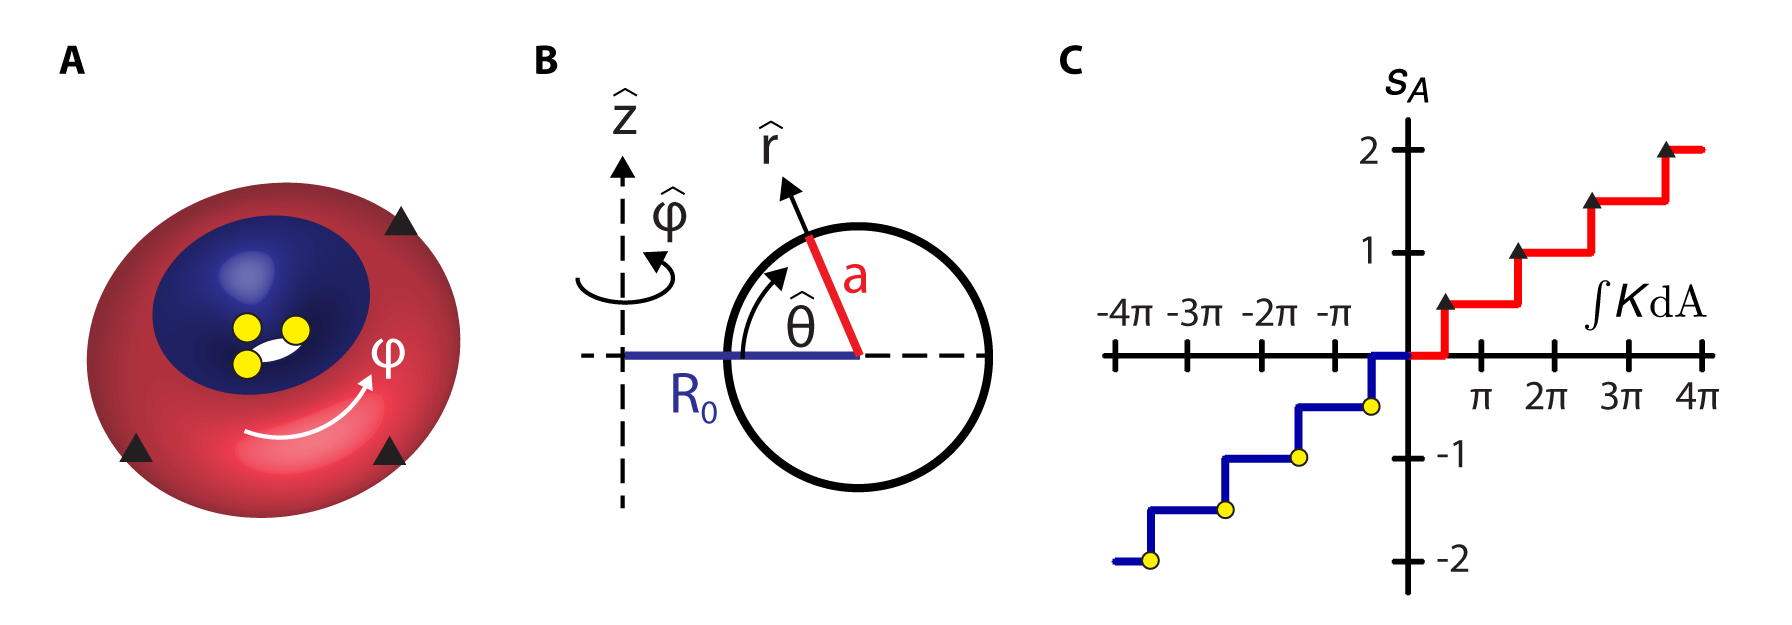
\includegraphics{figures/C3/Ch3-Figs_EqDefs.png}
  \caption{Curvature-induced defect unbinding for a nematic on a torus. (A) A schematic of a torus with 4 pairs of unbound pairs of $s = \pm 1/2$ defects. The 3 visible $s=+1/2$ defects are indicated by $\blacktriangle$ and the 3 visible $s = -1/2$ defects are indicated by ${\color{yellow} \bullet}$.
  The red region on the torus has $K >0$ and the blue region has $K<0$.
  (B) A schematic of a cross-section of a torus defining the toroidal coordinate system $\{r, \theta, \varphi \}$.
  A given torus is specified by its central circle radius, $R_0$ and its tube radius, $a$, which combine to form the aspect ratio, $\xi = R_0/a$.
  (C) Plot of topological charge vs integrated Gaussian curvature as $\varphi$ increases for the torus in (A).
  The red curve corresponds to integrating over the red region defined by $\theta \in [\pi/2,3 \pi/2]$ and the blue curve corresponds to integrating over the blue region defined by $\theta \in [-\pi/2,\pi/2]$. The positive slope indicates defect unbinding.}\label{f:3-EqDefs}
\end{figure}

In this chapter we consider a 2D extensile active nematic composed of microtubules driven by kinesin motors fueled by adenosine triphosphate (ATP) on the surface of a torus.
Since the torus has a handle, it has a genus of one and thus according to the Poincar\'e-Hopf Theorem written in Eq.~[INTRO] must have vanishing net topological charge.
We note that a nematic on a torus can satisfy this condition by either being defect-free or by having the same amount of positive and negative charge.
While strong spatial confinement or low activity can suppress the spontaneous formation of defect pairs in an active nematic~\cite{RN9,RN247}, we perform our experiments in the turbulent regime such that the torus is always populated with a sea of constantly moving $s = \pm 1/2$ defects that are dynamically created and annihilated.\\

Despite such chaotic and highly nonequilibrium dynamics, we find that on average, topological defects unbind and segregate in regions of oppositely-signed Gaussian curvature.
Notably, due to the chaotic dynamics and the averaging process, the topological charge ceases to be a discrete variable and instead approaches a continuous distribution.
In addition, contrary to equilibrium predictions~\cite{RN36,RN19,RN22,RN20,RN78}, we find that this active unbinding depends only on the local geometry and is independent of the system size and aspect ratio.
When also consider the defect species themselves and find that the average defect density depends inversely on Gaussian curvature over the majority of the toroidal surface.
We relate the dependence of the defect density on the Gaussian curvature to the creation rate of the defects; defects are created at a higher rate in regions of high curvature, leading to the inhomogeneous density.
We perform our studies with two different ATP concentrations and thus 2 different levels of activity and find that the defect unbinding and the defect density all depend on activity.
A numerical integration of the equation of motion of active nematic defects~\cite{RN11,RN8,RN9} performed by Luca Giomi and Dan Pearce at the University of Leiden confirms our experimental results and further illustrates that the defect unbinding can even be suppressed in the limit of high activity.
Furthermore, by using topological defects as micro-rheological tracers and quantitatively comparing our experimental and theoretical results, we are able to estimate the Frank elastic constant, the active stress, and the defect mobility of a microtubule-kinesin active nematic liquid crystal.
Overall, out results not only confirm the theory of topological defects on curved surfaces, but also demonstrate the surprising phenomenology that arises from adding activity to the interplay between geometry, topology, and order. Out work thus provides insights into the physics of partially ordered active matter and introduces a new avenue for the quantitative mechanical characterization of active fluids.\\


\section{Making active nematic toroids}
\subsection{Active nematic formulation}
We use the mictotubule-kinesin active nematic system pioneered by the Dogic Group at Brandeis University as published in references~\cite{RN3,RN27,RN9,RN135,RN134}.
Microtubules are long, hollow rods that self-assemble from dimers of the $\alpha$- and $\beta$-tubulin proteins~\cite{RN248}.
The $\alpha$/$\beta$-tubulin dimers polymerize end-to-end to form long chains that then polymerize laterally to create cylindrical structures with a helical wrapping of $\alpha$- and $\beta$-tubulin chains~\cite{RN248,RN249}, as depicted schematically in Figure~\ref{f:3-ActiveBuild}.
This structure gives microtubules a polarity with the (+) end associated with the exposed $\beta$-tubulin subunits and the (-) end associated with the exposed $\alpha$-tubulin subunits~\cite{RN248,RN249}.
While the microtubules serve as the mesogens of the active nematic, the activity comes from kinesin motor proteins bound in clusters to a streptavidin protein.
When in contact with a microtubule, kinesan ``walks'' along the microtubule in discrete steps from the (-) end towards the (+) end, hydrolyzing one ATP molecule into an adenosinediphosphate (ADP) molecule for every 8 nm step~\cite{RN250}.
Thus, a kinesin cluster in contact with two antiparallel microtubules will produce a sliding motion between the two microtubules as the motion of the kinesin motors on the microtubules will displace the two microtubules in opposite directions~\cite{RN4,RN3}.
Conversely, a kinesin cluster in contact with two parallel microtubules will simply walk along both microtubules in the same direction and thus produce no relative motion between the microtubules~\cite{RN4,RN3}. These two scenarios are illustrated schematically in Figure~\ref{f:3-ActiveBuild}(B).\\
\begin{figure}
  \centering
  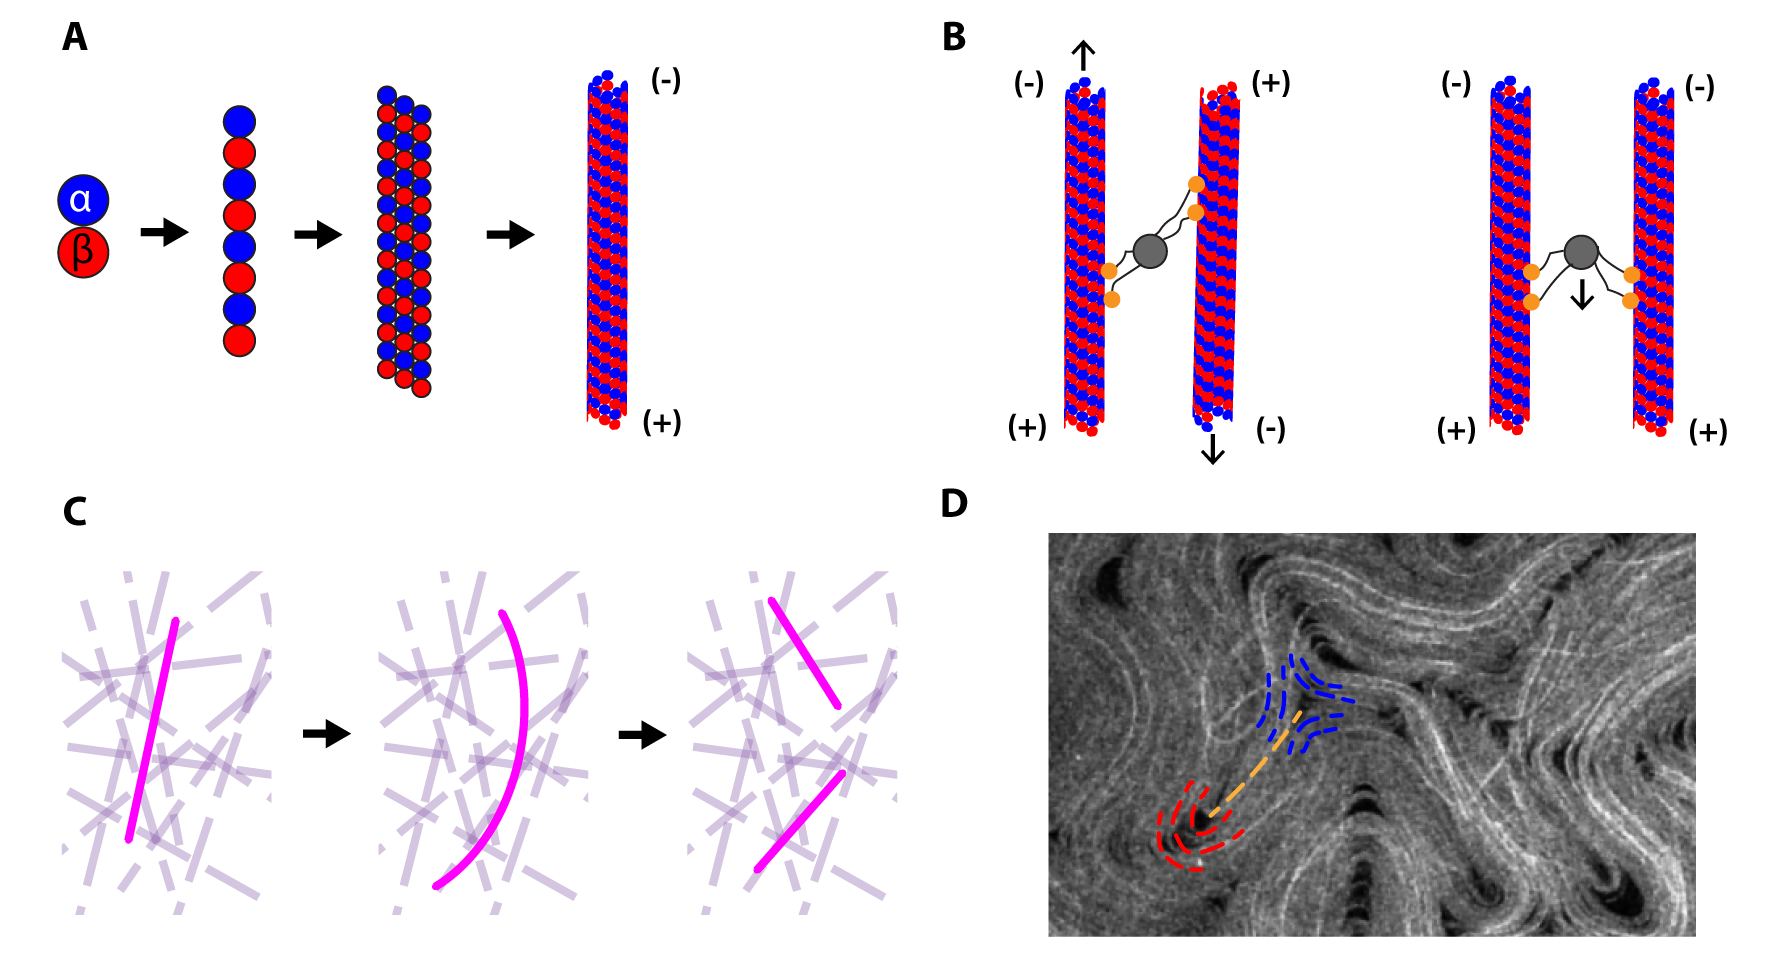
\includegraphics{figures/C3/Ch3-Figs_ActiveBuild.png}
  \caption{Microtuble-kinesin active nematic liquid crystal.
  (A) Schematic of tubulin polymerizing into a microtubule. The $\alpha/\beta$-tubulin dimers polymerize end-to-end to form chains which then polymerize laterally to form microtubules.
  The microtubule polarity is indicated on the schematic, with (-) associated to free $\alpha$-tubulin and (+) associated to free $\beta$-tubulin.
  (B) Kinesin, ${\color{yellow} \bullet}$, walks along microtubules from the (-) end to the (+) end.
  When kinesin are bound to streptavidin ${\color{gray} \bullet}$ to form clusters, these clusters can generate relative motion between two antiparallel microtubules.
  In contrast, parallel microtubules exhibit no relative motion, with the cluster simply translating itself in the shared (+) direction.
  (C) Microtubules and kinesin-streptavidin clusters bundles together by depletion form fibers that grow.
  When the concentration of fibers is high enough to form a viscoelastic network, individual fibers cannot grow freely and instead will buckle and fracture.
  (D) In the presence of a liquid-liquid interface, the fibers will deplete to the interface and undergo an isotropic-nematic transition, with the fiber direction giving the nematic director. Pictured is a fluorescence microscopy snapshot of an active nematic, where the microtubules are fluorescently labeled such that the fiber direction is apparent.}\label{f:3-ActiveBuild}
\end{figure}

Apart from the activity provided by the kinesin motors, the dominant interaction between the microtubules in an active nematic solution is the depletion interaction~\cite{RN251}, introduced via the presence of poly(ethylene glycol) (PEG, 20 kDa) as a depletant.
The depletion interaction ``bundles'' the microtubules together to form filaments that continuously grow due to the extensile interaction between microtubules provided by the kinesin motors~\cite{RN244,RN4,RN3}.
When the concentration of filaments in the active nematic solution is large enough, the filaments form a viscoelastic network~\cite{RN253,RN3}.
This network inhibits the growth of the filaments such that the filaments buckle at a critical length scale~\cite{RN253,RN3} and fracture into smaller fragments that recombine with other filaments, starting the growth-and-buckling process anew, as illustrated in Figure~\ref{f:3-ActiveBuild}(C).
In the presence of a liquid-liquid interface, the depletion interaction drives the filaments to the interface between the active nematic solution and outer phase, increasing the concentration such that the filaments locally align and undergo a transition to the nematic phase~\cite{RN3,RN135,RN134}, as seen in the example fluoresence microscopy image in Figure~\ref{f:3-ActiveBuild}(D), where the microtubules are fluorescently labeled such that the fiber direction is readily apparent.
Thus, the filament direction serves as the director for the 2D active nematic localized to the interface.
We note that the growth-and-buckling phenomenology of the active filaments is a physical consequence of the extensile dynamics and in the nematic phase is directly responsible for the bend instability and associated defect formation in the  microtubule-kinesin active nematics.
As the filaments buckle and fracture, an $s = +1/2$ and $s = -1/2$ defect pair is produced, with the defects nucleating at opposite ends of the fracture line~\cite{RN3,RN11}, as highlighted in the example image in Figure~\ref{f:3-ActiveBuild}(D)\fxnote{Fix the figure}.
Hence, with microtubules, kinesin-streptavidin complexes (K/SA), ATP, a depletant, and a liquid outer phase, we have the essential ingredients for an active nematic.\\

However, there are many more compounds in an active nematic solution that serve to enable measurements~\cite{RN3,RN135}, prolong activity~\cite{RN3,RN135}, and allow for a silicone-based outer phases~\cite{RN135}.
As mentioned earlier and shown in Figure~\ref{f:3-ActiveBuild}(D), the microtubules are fluorescently labeled such that the active nematic can be imaged with fluorescence or fluorescence confocal microscopy.
To prevent photobleaching and phototoxicity during imaging, the active solution contains trolox (Sigma, 238813) and two anti-oxidant solutions.
Anti-oxident solution 1 (AO1) is composed of glucose and dithiothreitol (DTT) and Anti-oxident solution 2 (AO2) is composed of glucose oxidase (Sigma, 238813) and catalase (Sigma, C40).
The active solution also includes an ATP regeneration system to keep the ATP concentration in an active nematic solution constant.
This system is driven by the enzyme mixture pyruvate kinase/lactate dehydrogenase (PK/LDH, Sigma, P-0294) which consumes phoshoenol pyruvate (PEP) to convert ADP to ATP at a rate faster than the K/SA hydrolyzes ATP to ADP~\cite{RN246}. \\

We note that when driven the the liquid-liquid interface, the active filaments do not ever contact the outer phase.
Instead, the interface is packed with a suitable surfactant such that the active nematic filaments deplete to the polar portion of the surfactant molecule.
In fact, the surfactant is then moved along the interface by the motion of the active filaments such that the viscosity of the outer oil phase significantly affects the dynamics of an active nematic~\cite{RN135}.
For a silicone-based outer fluid, we include the triblock copolymer Pluronic F127 (F127) composed of 2 hydrophilic PEG block attached to a central hydrophobic poly(propylene oxide) (PPO) block like PEG-PPO-PEG~\cite{RN252} to the active solution.
Finally, the solution is buffered using a specially designed microtubule buffer (M2B) to keep the enzymes and the motors in their preferred environments~\cite{RN3}.\\

For an experiment, we build the active nematic solution from stock solutions.
The stock solutions in their given compositions are {\bf bolded} such that PEP refers to the general compound while {\bf PEP} refers to the stock concentration/formulation as defined below:
\begin{itemize}
  \item[]{\bf M2B}: 80 mM 1,4-piperazinediethanesulphonic (PIPES) buffer~\cite{RN243} +2 mM MgCl$_2$ + 1mM egtazic acid (EGTA), pH 6.8
  \item[]{\bf PEP}: 200 mM in {\bf M2B}, pH 6.8.
  \item[]{\bf PK/LDH}: Used as purchased.
  \item[]{\bf ATP}: 50 mM in {\bf M2B}, pH 6.8
  \item[]{\bf DTT}: 0.5 mM in {\bf M2B}, pH 6.8
  \item[]{\bf trolox}: Used as purchased.
  \item[]{\bf MIX}: 67 mM MgCl$_2$ in {\bf M2B}
  \item[]{\bf PEG}: (20 kDa) 6\% w/w in {\bf M2B}
  \item[]{\bf F127}: 12\% w/w in {\bf M2B}
  \item[]{\bf glucose}: 300 mg/mL in 20 mM K$_2$HPO$_4$ + 70 mM KCl (pH 7.2)
  \item[]{\bf glucose oxidase}: 20 mg/mL in 20 mM K$_2$HPO$_4$ (pH 7.5)
  \item[]{\bf catalase}: 3.5 mg/mL in 20 mM K$_2$HPO$_4$ (pH 7.4)
  \item[]{\bf K/SA}: 0.175 mg/mL K401 + 0.1 mg/mL streptavidin (Invitrogen, S-888) + 12.5 mM imidazole (pH 6.8) + 1 mM MgCl$_2$ + 0.75 mM DTT + 12.5 mM ATP in {\bf M2B}. K401 consists of 401 amino acids of the N-terminal motor domain of \emph{D.~melanogaster} kinesin purified as previously published~\cite{RN3}.
  \item[]{\bf MT}: 8 mg/mL tubulin labeled with AlexaFluor 647 at 28\% labeling efficiency in {\bf M2B}. Tubulin was purified as previously published~\cite{RN243}.
\end{itemize}
The stock solutions were prepared by the Dogic Group at Brandeis and then shipped to Georgia Tech.
We pipetted the stock solutions as received into aliquots suitable to make 100 $\upmu$L of active nematic solution.
The aliquots are stored in a freezer at $-80^o$ C to prevent degradation of the active compounds.
Prior to each experiment, we remove a set of aliquots from the freezer, quickly thaw the aliquots to room temperature by holding them in our closed hands, and then place all the aliquots on ice except for the MT aliquot.
We leave the MT aliquot out at room temperature so that the tubulin can self-assemble into microtubules.
The polymerization of microtubules is temperature-dependent, with tubulin polymerizing to form microtubules at room temperature and microtubules depolymerizing into tubulin at low temperature~\cite{RN3}.
We then make the initial mixtures and the pre-solution according to the recipe in Table~\ref{t:3-recipe}, leaving the pre-solution on ice.
We wait at least 90 minutes after bringing the MT aliquot to room temperature before mixing the MT with the pre-solution to form the final active nematic solution as specified in Table~\ref{t:3-recipe}.
Note that we bring the pre-solution to room temperature before adding in the microtubules such that the microtubules do not depolymerize when they are added to the pre-solution.
Once we mix the final solution together, we perform our experiments and observe the active nematic until the activity ceases.

\begin{table}[ht]
  \centering
  \caption{Recipe for 100 $\upmu$L active nematic solution}
  \begin{tabular}{|r l|}
    \hline
    \multicolumn{2}{|c|}{Initial mixtures}\\
    \hline
    A01 & 1.5 $\upmu$L {\bf DTT} + 1.5 $\upmu$L {\bf glucose} \\
    A02 & 1.5 $\upmu$L {\bf glucose oxidase} + 1.5 $\upmu$L {\bf catalase} \\
    ATP2 & 2 $\upmu$L {\bf ATP} in:\\
    & \quad 18 $\upmu$L {\bf M2B} for a 10x dilution.\\
    & \quad 38 $\upmu$L {\bf M2B} for a 40x dilution.\\
    \hline
    \multicolumn{2}{|c|}{Pre-solution}\\
    \hline
    2.21 $\upmu$L & A01\\
    2.21 $\upmu$L & A02\\
    2.83 $\upmu$L & ATP2\\
    2.83 $\upmu$L & {\bf PK/LDH} \\
    4.83 $\upmu$L & {\bf MIX}\\
    10.00 $\upmu$L & {\bf trolox}\\
    13.33 $\upmu$L & {\bf PEP}\\
    13.33 $\upmu$L & {\bf PEG}\\
    16.67 $\upmu$L & {\bf F127}\\
    6.67 $\upmu$L & {\bf K/SA}\\
    8.40 $\upmu$L & {\bf M2B}\\
    \hline
    \multicolumn{2}{|c|}{Active nematic solution}\\
    \hline
    83.33 $\upmu$L & Pre-solution (full volume is 83.33 $\upmu$L)\\
    16.67 $\upmu$L & {\bf MT}\\
    \hline
  \end{tabular}
  \label{t:3-recipe}
\end{table}


\subsection{Flat sample confirmation}
Upon receiving the stock solutions, we first made a bulk active gel according to the procedures published in ref.~\cite{RN3} to confirm the integrity of the solutions through the shipping process.
To make a gel, we have to construct a sample chamber where the depletion interaction cannot drive the bundles to aggregate on the walls of the chamber.
We build the sample chamber from a glass coverslip attached via two-sided tape to a microscope slide to form a rectangular channel, as previously published~\cite{RN3}.
Prior to construction, we coat the coverslip and microscope slide with polyacrylamide brushes such that the PEG can penetrate between the brushes, keeping the depletion interaction from driving the active filaments to the surface, where they would adsorb to the glass~\cite{RN3}.
We coat the coverslip and microscope slide according to the published protocol~\cite{RN3}, reproduced in Appendix~\ref{a:B}.\\

To make the rectangular sample chambers from the polyacrylamide-coated glass, we cut strips of 2-sided tape such that the are $\approx1$ mm wide and longer than the coverslip.
We then affix the tape strips to the microscope slide in parallel with $\approx 2$ mm between the edges of adjacent strips, and then stick the coverslip onto the tape to create a parallel series of rectangular channels.
It is important to press firmly such that the tape is firmly adhered to both the coverslip and the glass.
Finally, we fill the channels with the active solution using capillary action and seal the ends of the channel with epoxy.
A schematic of the sample chamber and assembly process is shown in Figure
The samples are now ready to be imaged using fluorescence or fluorescence confocal microscopy. \\
\begin{figure}
  \centering
  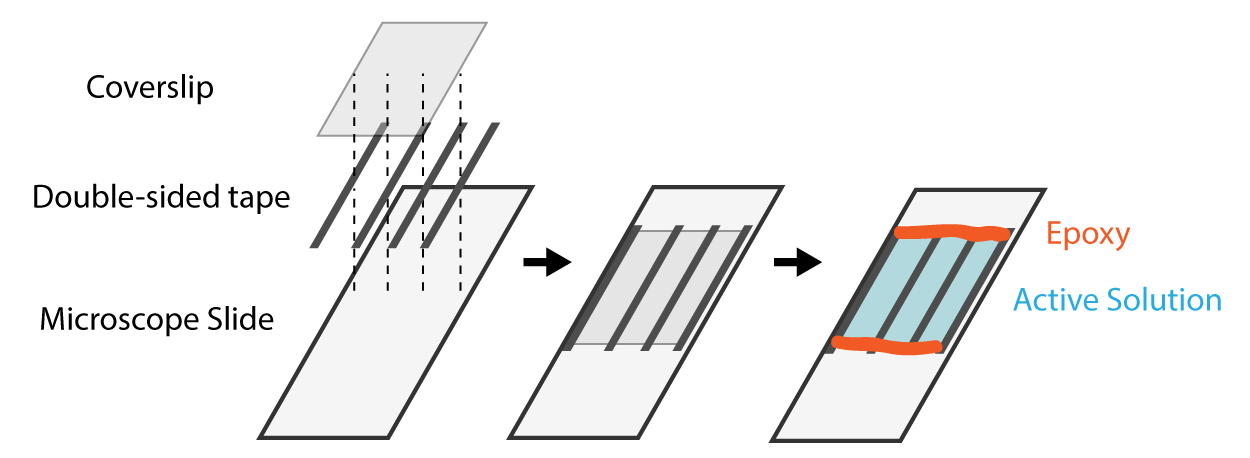
\includegraphics{figures/C3/Ch3-Figs_GelSampleChamber.png}
  \caption{Schematic and asembly of a sample chamber for an active gel.}
  \label{f:3-SampleChamber}
\end{figure}

We confirmed that the stock solutions received produced an active gel with fluorescent active filaments that grew and fractured.
The activity in the gel sample appeared constant for the entirety of its  $\approx 24$ hr lifespan.
The observed behavior qualitatively agreed with previously published behavior by the Dogic group~\cite{RN3}.


\subsection{Making toroidal droplets}
With the integrity of the active solution confirmed, we turn to making stable toroidal droplets with our active solution.
We generate our toroidal droplets following the procedure detailed in Refs.~\cite{RN29,RN47,RN257}.
Briefly, the setup consists of a rotating stage holding a cuvette containing the continuous, or outer phase, and a syringe holding the dispersed, or inner phase connected to a needle inserted into the cuvette.
We control the angular velocity of the rotation $\omega$, by driving the rotating the stage with a motor powered by a constant voltage source.
We control the position of the needle in the cuvette with a micromanipulator and we control the flow rate and volume of the inner phase with a syringe pump.
In addition, we place a camera below the rotation stage such that we can image the droplet generation process.
This setup is depicted schematically in Figure~\ref{f:3-MakeTorus}(A)
We insert the needle into the cuvette offset from the center of rotation such that pumping the inner phase into the cuvette while the cuvette is rotating will generate a curved jet, as shown in the example image in Figure~\ref{f:3-MakeTorus}(B).
Provided that we rotate fast enough such that the curved jet closes upon itself before it undergoes breakup, we form a toroidal droplet, as shown in the example image in Figure~\ref{f:3-MakeTorus}(C).
This condition is a balance of two timescales: (i) the timescale required to undergo breakup, $t_b \approx \mu_o a_{jet} f(\mu_i/\mu_o)/\gamma$, where $\mu_o$ is the viscosity of the outer phase, $\mu_i$ is the viscosity of the inner phase, $a_{jet}$ is the radius of the jet, and $\gamma$ is the interfacial tension between the inner and outer phases;
  and (ii), the timescale required to close the curved jet onto itself, $T = 2\pi/\omega = 2 \pi R_{tip}/U$, where $R_{tip}$ is distance from the center of rotation the the needle, as depicted in Figure~\ref{f:3-MakeTorus}(C)\fxnote{fix figure} and $U$ is the linear velocity of the continuous phase at the needle.
Equating the two timescales and rearranging terms allows us to express this condition in terms of the Capillary number of the outer phase like $\textup{Ca}_o > (2 \pi / f(\mu_i/\mu_o))R_{tip}/a_{jet}$ ,where $\textup{Ca}_o = \mu_c U/\gamma$ a dimensionless group comparing the viscous stresses to the surface tension stresses.
We note that $a_{jet} \approx a_{tip}$, the radius of the needle.
Experimentally, it has been found that $\textup{Ca}_o > 2.2 R_{tip}/a_{tip}$ for $\mu_o = 5000$~mPa~s and $\mu_i = 1$~mPa~s in order to form a torus~\cite{RN29}.
In practice, we simply look at the video of the process to verify that our chosen parameters generates a jet that closes in upon itself before breaking.
To control the size and aspect ratio of the toroidal droplet, we tune $R_0$ by changing $R_{tip}$ and $a$ through the total injected volume. \\
\begin{figure}
  \centering
  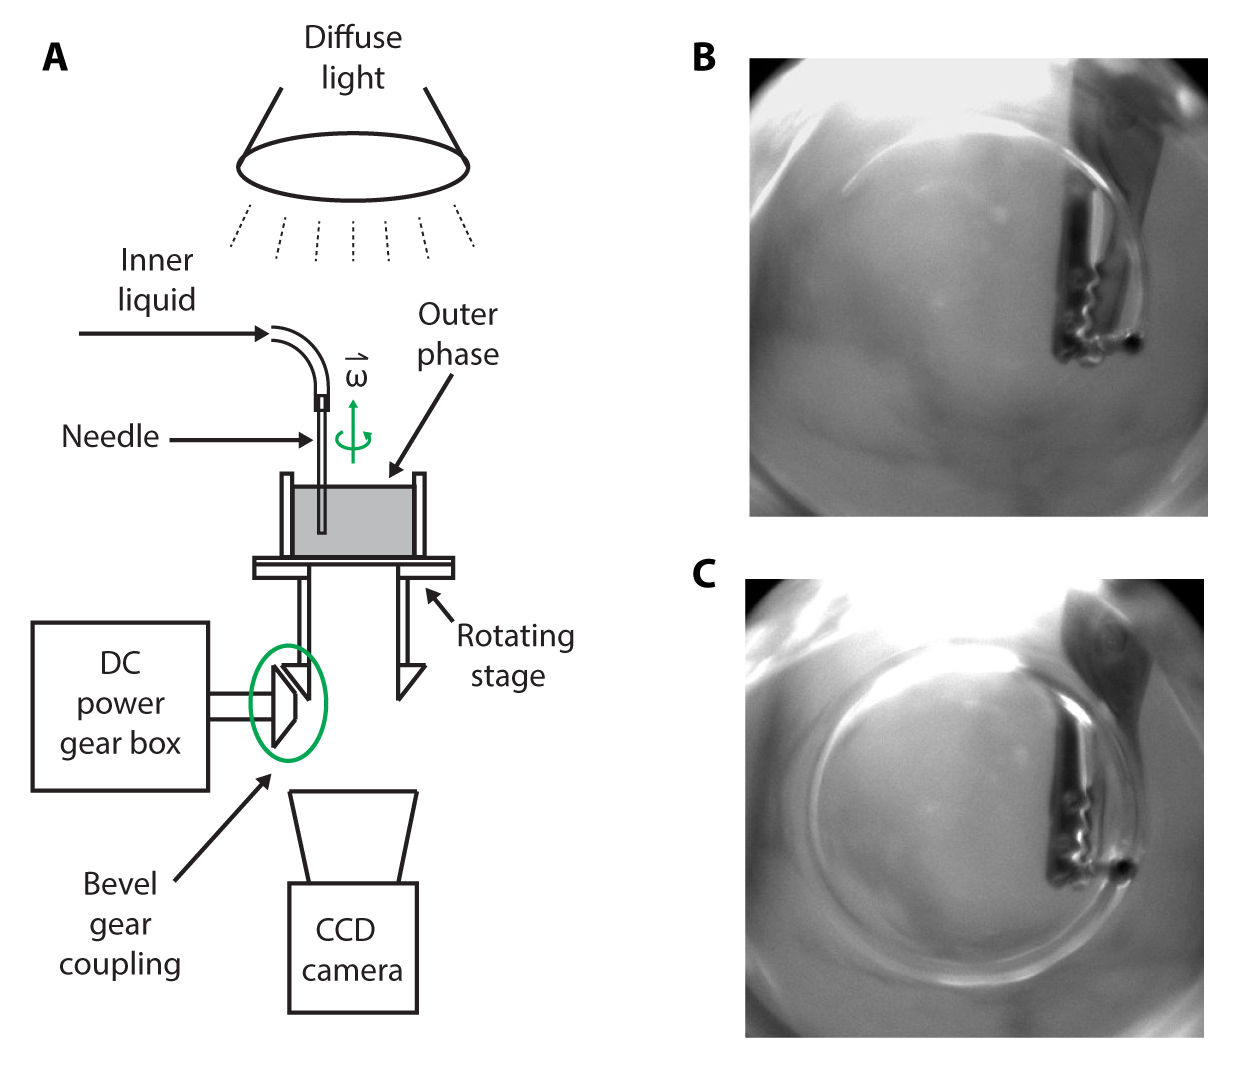
\includegraphics{figures/C3/Ch3-Figs_MakeTorus.png}
  \caption{Making toroidal droplets.
  (A) Schematic of the apparatus used to make toroidal droplets.
  The inner fluid is injected into a cuvette on a rotating stage.
  The stage is driven by a DC motor and the entire process is imaged from below with a CCD camera.
  (B) A curved jet pulled from the needle by the viscous drag of the rotating bath.
  (C) A toroidal droplet formed when the curved jet in (B) closed upon itself.}\label{f:3-MakeTorus}
\end{figure}

Toroidal droplets generated in a simple fluid are unstable due to the influence of surface tension.
Surface tension acts to minimize the interfacial area between two immisicble fluid phases, hence the ubiquity and stability of spherical droplets in nature; the sphere minimizes the surface area for a given volume~\cite{RN178}.
The physics behind the surface tension stress at an interface comes through the Laplace pressure $\Delta P$, describing the pressure drop across a fluid-fluid interface~\cite{RN178}:
\begin{equation}\label{e:3-LapPres}
  \Delta P = P_i - P_o = 2 \gamma (- H),
\end{equation}
where $P_i$ is the pressure in the inner fluid phase, $P_o$ is the pressure in the outer fluid phase, and $H$ is the mean curvature of the interface.
Recall that $H = \textup{det}\big \{ \mathbf{L} \big \}$, where $\mathbf{L}$ is the Weingarten Matrix from Eq.~[INTRO]\fxnote{ref INTRO} defined such that the mean curvature of a sphere with radius $r$ choosing an outward-facing normal is $H = -1/r$ everywhere on the surface of the sphere.
Thus, the Laplace pressure tells us that a spherical droplet has greater pressure on the inside than on the outside, and that due to its constant mean curvature, the pressure inside the droplet is also constant such that the droplet is stable.
However, we know that $H$ for a torus varies along the surface such that the pressure inside the torus must also vary.
This intrinsic pressure difference creates the flow inside a fluid torus responsible for the shrinking instability in toroidal droplets, where the handle shrinks smoothly until it closes and the toroidal droplet becomes a spherical droplet~\cite{RN29,RN255}.
In addition, the Laplace pressure can also cause the tube of a toroidal droplet to break up reminiscent of the Rayleigh-Plateau instability such that the toroidal droplet breaks into one or more spherical droplets~\cite{RN29,RN256}.
While the study of the fluid modes in nontrivial topologies is interesting in its own right and has led to interesting insights into fluid phenomena such as charged jets~\cite{RN256} and viscous fingering~\cite{RN254}, we are more concerned with creating a stable toroidal droplet. \\

As the surface tension stress is responsible for destabilizing the toroidal droplet, to stabilize a toroidal droplet we need to counter the surface tension stress.
To do so, we make our toroidal droplets using a yield-stress material as the outer phase~\cite{RN47,RN258}.
Briefly, a yield-stress material has a threshold stress such that the material responds like an elastic solid to imposed stresses less than the yield-stress and flows like a viscous liquid to imposed stresses greater than the yield-stress.
Thus, provided that the yield-stress is greater than the surface tension stress, the toroidal droplet will be unable to transform to a spherical droplet and will be stable indefinitely.
Since the surface tension stress is given by the Laplace pressure, we see that balancing the Laplace pressure and the yield stress, $\tau_c$, will give us a critical radius of curvature, $R_c$, determining the stability of a toroidal drop, $\gamma/\tau_c \sim R_c$.
If the smallest radius of curvature on a toroidal drop is larger than $R_c$, the toroidal droplet will be stable --- generally, the smallest radius of curvature on a torus is the tube radius.
However, for toroids with $\xi \sim 1$, the radius of the handle can be the relevant lengthscale determining the stability of a toroidal droplet.
Since the active nematic solution is aqueous, we use an oil-based yield-stress material, DC-9041 (Dow Corning), a silicone elastomer.
To tune the yield stress, we dilute pure DC-9041 with 10~cSt PDMS oil (Clearco).\
We dilute to 74\%~--~77\% w/w DC-9041 to form stable active nematic toroids with tube radii from 150~$\upmu$m~--~300~$\upmu$m.\\

Making a toroidal droplet in a yield-stress material has some key differences to making a toroidal droplet in a viscous fluid.
Notably, the yield-stress material is only fluid-like in regions where the stress is greater than the yield-stress.
Thus, for best results, we need to pre-shear the yield-stress medium such that the greatest possible volume of yield-stress material is fluidized.
We do this by letting the cuvette rotate with the needle inserted for up to 30 s before we begin pumping the inner liquid into the cuvette.
While a pre-shear is not strictly necessary to form a toroidal droplet, the cross-sections of the tubes of toroidal droplets made with a pre-shear are generally more circular than toroidal droplets made with minimal pre-shear.
This is because the wider the volume of fluidized yield-stress material, the less the pumped volume ``climbs'' up the needle.
In addition, adding a pre-shear generally helps the overall toroidal droplet be more axisymmetric.
We also find that making toroidal droplets close to the free-surface of the yield-stress material helps to reduce climbing, but the physical reason for this is unclear.\\

For general experiments with toroidal droplets where there is a large amount of the inner phase available, we simply fill the syringe with the inner phase.
However, for the active experiments, we have only 100~$\upmu$L of active solution per experiment, which is not enough to even fill the Luer-lock syringe tips we use to connect a syringe to the tubing.
To accommodate the low sample volume, we fill the syringe with mineral oil (xx cSt, XXX)\fxnote{GET MO source} as a dummy fluid and increase the length of the tubing between the syringe and the needle such that the volume of tubing is greater than $100$~$\upmu$L.
We pump the dummy fluid until it fills the tubing, insert the filled tubing into the container holding the active nematic solution, and the withdraw the dummy fluid to pull the active nematic solution into the tubing.
Once the active nematic solution is loaded into the tubing, we make toroids as if it were any other inner phase.
It is important to make sure that the tubing is entirely full of mineral oil such that there is no air at the interface between the dummy liquid and the active nematic solution.
Air bubbles in the tubing will inhibit forming high-quality toroidal droplets as the air bubble acts as a ``spring'' in the fluid system, introducing significant ``lag'' between the start and stop of the syringe pump and the beginning and end of the fluid flow from the needle.
In addition, it is important to withdraw the dummy fluid slowly ($\approx 1$~mL/s) when loading the active nematic solution to prevent an emulsion between the active fluid and the dummy fluid forming in the tube.\\




\section{Imaging active nematic toroids}
Once the active nematic toroidal droplet is made, we let the droplet rest for 2~--4~4~hours to ensure the nematic is fully formed on the surface of the toroidal droplet.
We then image the droplet via fluorescence confocal microscopy (Nikon A1R or Zeiss LSM 700) until the activity ceases.
This typically occurs between 6~--~10~hours after making the toroidal droplet.


\subsection{Confocal fluorescence microscopy}
Unlike traditional wide-field microscopy, confocal microscopy allows us to image individual planes in the image such that we can construct a 3D representation of the sample~\cite{RN260}.
Regardless of the illumination source, confocal microscopy functions by placing an aperture in front of the detector at a confocal plane to the focal plane in the sample~\cite{RN259}.
Thus, only light from the focal plane will pass through the aperture; light from any other plane in the sample will be out of focus in the plane of the aperture and thus will not pass through the aperture.
Typically, the focal plane is changed in the sample by translating the microscope stage up and down.
Since the introduction of scanning confocal microscopy, and especially scanning laser confocal fluorescence microscopy, confocal microscopy has seen widespread adoption and is now a standard technique in multiple fields~\cite{RN261,RN262,RN260}.
Here, the illumination mode is epifluorescent, such that a laser beam is emitted through the objective and incident on a portion of the sample.
The illuminated portion of the sample then fluoresces and the output intensity from the focal plane is recorded.
This process is enhanced with a dichroic mirror and a pair of filters such that both the illumination source and the emitted light pass through the objective, but only the emitted light is passed to the detector.
With a tight laser beam and a set of mirrors to scan the laser beam over the sample, the emitted intensity in the focal plane can be highly localized such that the spatial resolution in the focal plane is set by the size of the laser spot~\cite{RN260}.
This reduces the impact of photobleaching, but more importantly allows the user to `zoom'' into the sample without changing the objective magnification simply by changing the size of the laser spot and detector optics such that a smaller scan area with higher spatial resolution in a given focal plane still illuminates the entire detector.
We note that the $z$-resolution between focal planes is still set by the diffraction limit of the emitted light, such that the only way to meaningfully improve the $z$-resolution is to change the objective.
Coupling confocal microscopy to fluorescence microscopy not only improves signal-to-noise ratio, but also allows us to selectively image only the dyed portion of the sample.
In our case, this corresponds to imaging only the active filaments.
Thus, we can acquire a 3D image stack showing only the active nematic depleted to the toroidal surface.


\subsection{Confocal setup and parameters}
Both of the confocals we use are scanning laser confocal microscopes.
Procedurally, both microscopes scan the image plane with a focused laser beam while recording the output intensity, adjust the height of the stage to change the focal plane, and then repeat the process until the image stack is acquired.
While the image stack can be thought of in terms of 3D voxels, the $z$-resolution between focal planes is less than the $xy$-resolution in the focal plane such that it is more convenient to think of the image acquisition as a stack of 2D images.
We note that we are inherently restricted to only imaging the lower half of the toroidal droplet due to refraction effects.
The light emitted from the upper half of the toroidal droplet travels through the aqueous active solution and then is refracted by the curved interface between the active solution and the yield-stress material.
In contrast, the light from the lower portion of the toroid is emitted directly into the yield-stress material such that it's light path is unaffected by refraction.
However, even though we can in principle image up to the midpoint of the torus, in practice we typically stop our image stack below the midpoint.
This is because the time required to adjust the stage height is the slowest portion of the imaging process for both of the confocal microscopes we use.
Since we wish to acquire as many frames as possible to increase the amount of data we have for each toroid, we must must balance the time required to take an image stack versus the size of the image stack.\\

The microtubules are dyed with AlexaFluor 647, which has en excitation peak of 651~nm and an emission peak of 667~nm~\cite{RN264}.
Thus, we use a 633~nm laser as our illumination source and a Cy5 filter set such that only the emitted light reaches the detector.
The Cy5 filter set includes a 590~--~650~nm bandpass excitation filter, a 660~nm longpass dichroic mirror, and a 663~--~738~nm emission filter~\cite{RN263}.
The filters and mirror are designed with steep passband transitions such that the quoted ranges are good representations of the passband.
Note that for illumination with a laser, the excitation filter is unnecessary, but is standard when purchasing the filterset.
The excitation filter is necessary in wide-field fluorescence microscopy when illuminating with a white-light source.\\

While the two confocal microscopes we use operate the same, there are key differences in the detection that affects measurement protocol as we affects the quality of the data.
The Zeiss microscope uses standard photomultiplier tubes (PMT) as the detector.
Unfortunately, standard PMTs do not detect wavelengths above 600~nm well, as the quantum efficiency of the detector decreases with increasing wavelength and is typically below 10\% in that wavelength range~\cite{RN263}.
This means that we have to increase the intensity of the laser, increase the gain on the detector, and even average two scans of each image plane in order to increase the signal-to-noise ratio to an acceptable level.
As a result, data from the Zeiss microscope take longer to collect and the active nematic exhibits mild photobleaching for long acquisitions.
However, we note that the photobleaching is mild enough that it does not appreciably affect our data analysis. \\

In contrast, the Nikon microscope uses a Gallium Arsenide Phosphide (GaAsP) PMT in conjunction with standard PMTs to increase the quantum efficiency of the detector suite for larger wavelengths.
GaAsP PMTs maintain a roughly constant quantum efficiency of $\approx 50$\% up to 700~nm~\cite{RN263}.
Thus, we can keep both the laser power and detector gain low while still only needing a single scan of the image plane to acquire a higher quality image stack than we get from the Zeiss microscope.
We therefore can acquire image stacks with a higher time resolution, a higher image quality, and with no noticeable photobleaching when using the Nikon microscope.\\

We set up a measurement as follow.
First, we place the sample on the microscope stage and and find the droplet by eye using standard brightfield microscopy.
We then set up the confocal such that appropriate laser and filter set are chosen.
Next, we set the microscopes to scan the image plane and display the output in real time.
We move the stage to find the bottom and the sample and then move the stage to determine the highest plane that we will measure.
As a rule of thumb we aim for one image stack to take 30~--~50~s to acquire.
This corresponds to roughly 15~--~25 image planes, depending on the microscope used to acquire the data. \\

Now that we have set up the size of the image stack, we turn to tuning the laser intensity and gain to produce the highest quality images.
We first find the image plane with the brightest intensity, and manipulate the intensity and gain such that at most $\approx 5$\%  of the pixels are saturated.
While a higher laser power and lower gain will produce better quality images, setting the laser power too high can lead to photobleaching for long time measurements.
Thus, we generally keep the gain roughly halfway between the minimum and maximum values and then adjust the laser power accordingly.
If we are on the Zeiss microscope, we set the microscope to scan each image plane twice and average the measurements such that we can reduce the overall laser power to minimize photobleaching.
We then go to the bottom plane and set an offset corresponding to an intensity floor for the measurement.
Pixels with an intensity below the offset are set to 0.
This helps to remove some of the thermal noise in the image; in practice, we have enough signal that this parameter is does not really matter.\\

Once these parameters have been set, we turn on the Perfect Focus System to eliminate the effect of thermal and mechanical drift in the measuring system.
Thermal and mechanical drift in the measuring system means that over time the measured distance between the objective and a given reference plane in the sample will change.
This will result in the physical sample volume imaged by the confocal changing over time.
The Perfect Focus System corrects this by maintaining the distance between a specified reference plane and the objective with incredibly high accuracy.
The microscope then resets its zero to the reference plane before every scan through the image stack and thus will never accumulates error due to drift.
Finally, we set the microscopes to image continuously for 12 hours, starting the next image stack as soon as it finishes the previous stack until the 12 hours have expired.
We note that files imaged for longer than 12 hours can be difficult to open due to their large size, even on the computer associated to the microscope.\\

Once the image acquisition is finished, we crop the raw confocal time series to only include the portion where the toroidal droplet is active.
We save this cropped version in single multi-page \texttt{.tiff} file including the metadata concerning acquisition parameters.
This standardizes the data format between the different microscopes to make it easier to read in to the computer.


\subsection{Passing confocal data into MATLAB}
The core routine to load the image stack into MATLAB comes from the \texttt{bioformats} toolbox put out by the Open Microscopy Environment~\cite{RN265}.
The Open Microscopy Environment maintains the open-source \texttt{OME-TIFF} image format for microscopy data.
The \texttt{bioformats} toolbox allows us to call the imaging parameters such as pixel-to-length conversions, framerate, etc., as well as access the total times series of image stacks as a 3 dimensional array in MATLAB.
The data are stored in image planes in the order they were taken such that the effect is concatenating the time-series of image stacks along the $z$ dimension in the order they were taken.
Thus, to locate a specific image stack you have to know which stack in the time series you want as well as the number of planes in each image stack.
Since the entire image series from the confocal can be up to 8~Gb, we first extract the relevant data and then remove the image series from memory so that we have the ability to analyze the data.\\

We first determine the surface of the toroidal droplet by averaging all the image stacks together and then applying an intensity threshold.
Since we have fluorescence confocal data where the fluorescent media has depleted to the surface of the torus, averaging all of the image stacks together creates a clear intensity image of the toroidal surface as both transient structures in the bulk as well as the filamentary structure of the active nematic is washed out in the averaging process.
We next threshold the data to binarize the image stack and reduce the thickness of the surface in the binary stack.
Since there are a large range of threshold values that do not change the output surface and it is easy to check the result of an applied threshold, we determine this threshold value by hand.
From the binarized 3D array, we look at every $xy$ position and determine the lowest $z$ value that contains a nonzero value.
We take this $z$ value to be the height $h$ of the toroidal surface record it in an array such that we have a Monge parameterization of our surface, $h = f(x,y)$~\cite{RN23}. \\

We next consider the intensity stack for each time point and perform a maximum intensity projection into the $xy$-plane with the caveat that the only consider pixels within $\pm 5$ planes of the height at each individual point.
This process largely prevents transient bright filaments in the bulk from affecting our measurements.
Thus, we now have recorded our surface and reduced our data from a time-series of 3D image stacks to a time-series of 2D images such that we have the intensity $I = f(x,y,t)$.
Finally, we clear the raw confocal data from memory and work to (i), determine the director and defects from the intensity projections, and (ii), calculate the surface curvature and surface normals using $h(x,y$).




\section{Determining director and defects}
In the intensity projection of a confocal stack at a time $t_0$, $\mathbf{n}$ is given by the direction of the microtubule bundles.
This direction is obtained from the greyscale image by finding the direction along which the intensity fluctuates the least for each pixel using a technique called coherence-enhanced diffusion filtering (CEDF)\cite{RN30}.
We illustrate this technique with an example analysis of the intensity projection shown in Figure~\ref{f:3-CEDF2}(A).


\subsection{Coherence-enhanced diffusion filtering}
To begin with, the original intensity image $I = I(x,y,t_0)$ is denoised using a Gaussian blur of standard deviation $\sigma$ and side length $6 \sigma -1$ to lessen contributions to the intensity fluctuations from random noise, giving us the blurred image $I_{\sigma}$.
The result of blurring the example full-stack image as well as the inset isolated defect pair in Figure~\ref{f:3-CEDF2}(A) is seen in the main image and inset of Figure~\ref{f:3-CEDF2}(B), respectively.
This blur was performed using a $5 \textrm{ px} \times 5 \textrm{ px}$ Gaussian filter with $\sigma= 1$ px.\\

Next, the gradient tensor for $I_{\sigma}$ is calculated for each pixel:
\begin{equation}
(\nabla I_{\sigma})(\nabla I_{\sigma})^T =
\begin{bmatrix}
(\nabla_x I_{\sigma})(\nabla_x I_{\sigma}) & (\nabla_x I_{\sigma})(\nabla_y I_{\sigma}) \\
(\nabla_y I_{\sigma})(\nabla_x I_{\sigma}) & (\nabla_y I_{\sigma})(\nabla_y I_{\sigma})
\end{bmatrix}.
\end{equation}
Since the microtubule bundles have head-tail symmetry, we cannot use the gradient vector alone to define the bundle orientation as the vector has a defined head and tail.
The rank-2 gradient tensor is symmetric and is the same whether it is constructed with the gradient vector or the negative gradient vector.
Thus, we use the gradient tensor to ``remove the head'' from the gradient vector.
We now define the coherence direction of a rank-2 tensor as the direction of the eigenvector associated with the smallest eigenvalue.
The coherence direction represents the direction along which the spatial intensity fluctuations are the weakest and is periodic on the interval $[0^{\circ}, 180^{\circ})$.
The coherence direction calculated for the gradient tensor of each pixel for $I_\sigma$ shown in the main image and inset of Figure~\ref{f:3-CEDF2}(B) is seen in the main image and inset of Figure~\ref{f:3-CEDF2}(C), where the orientation of the coherence direction on the interval $[0^{\circ}, 180^{\circ})$ measured CW off of the horizontal axis has been mapped to the greyscale values $[\textrm{black}, \textrm{white})$ .
We see that there are still too many fluctuations in the coherence directions shown in Figure~\ref{f:3-CEDF2}(C) to determine $\mathbf{n}$.\\

The following step seeks to remove small-scale fluctuations in the coherence direction by averaging once more.
Here, we perform a component-wise average of the gradient tensor for each pixel to find the structure tensor for each pixel.
This operation can be written as:
\begin{equation}
K_{\rho} \ast (\nabla I_{\sigma})(\nabla I_{\sigma})^T =
\begin{bmatrix}
K_{\rho} \ast ( \nabla_x I_{\sigma})(\nabla_x I_{\sigma}) & K_{\rho} \ast (\nabla_x I_{\sigma})(\nabla_y I_{\sigma}) \\
K_{\rho} \ast (  \nabla_y I_{\sigma})(\nabla_x I_{\sigma}) & K_{\rho} \ast (\nabla_y I_{\sigma})(\nabla_y I_{\sigma})
\end{bmatrix},
\end{equation}
where $K_{\rho}$ is a Gaussian filter with standard deviation $\rho$, where $\rho$ should be about the size of the relevant coherence feature in the image.
If $\rho$ is too small, the coherence directions of the structure tensor will resemble those from the gradient tensor, while if $\rho$ is too large the desired coherence features will be washed out by the averaging.
The coherence direction of the structure tensor calculated with $\rho = 5$ px and filter size $29\textrm{ px } \times 29$ px for each pixel of $I_{\sigma}$ seen in the main image and inset of Figure~\ref{f:3-CEDF2}(B) is shown in the main image and inset in Figure~\ref{f:3-CEDF2}(D), respectively.
As before, the orientation on the interval $[0^{\circ}, 180^{\circ})$ measured CW off of the horizontal axis has been mapped to the greyscale values $[\textrm{black}, \textrm{white})$.
 We take this output of the coherence direction of the structure tensor for each pixel as the local ``molecular director'' $\mathbf{u}$, representing the local orientation of the active nematic.
\newpage
\begin{figure}[h!]
  \centering
  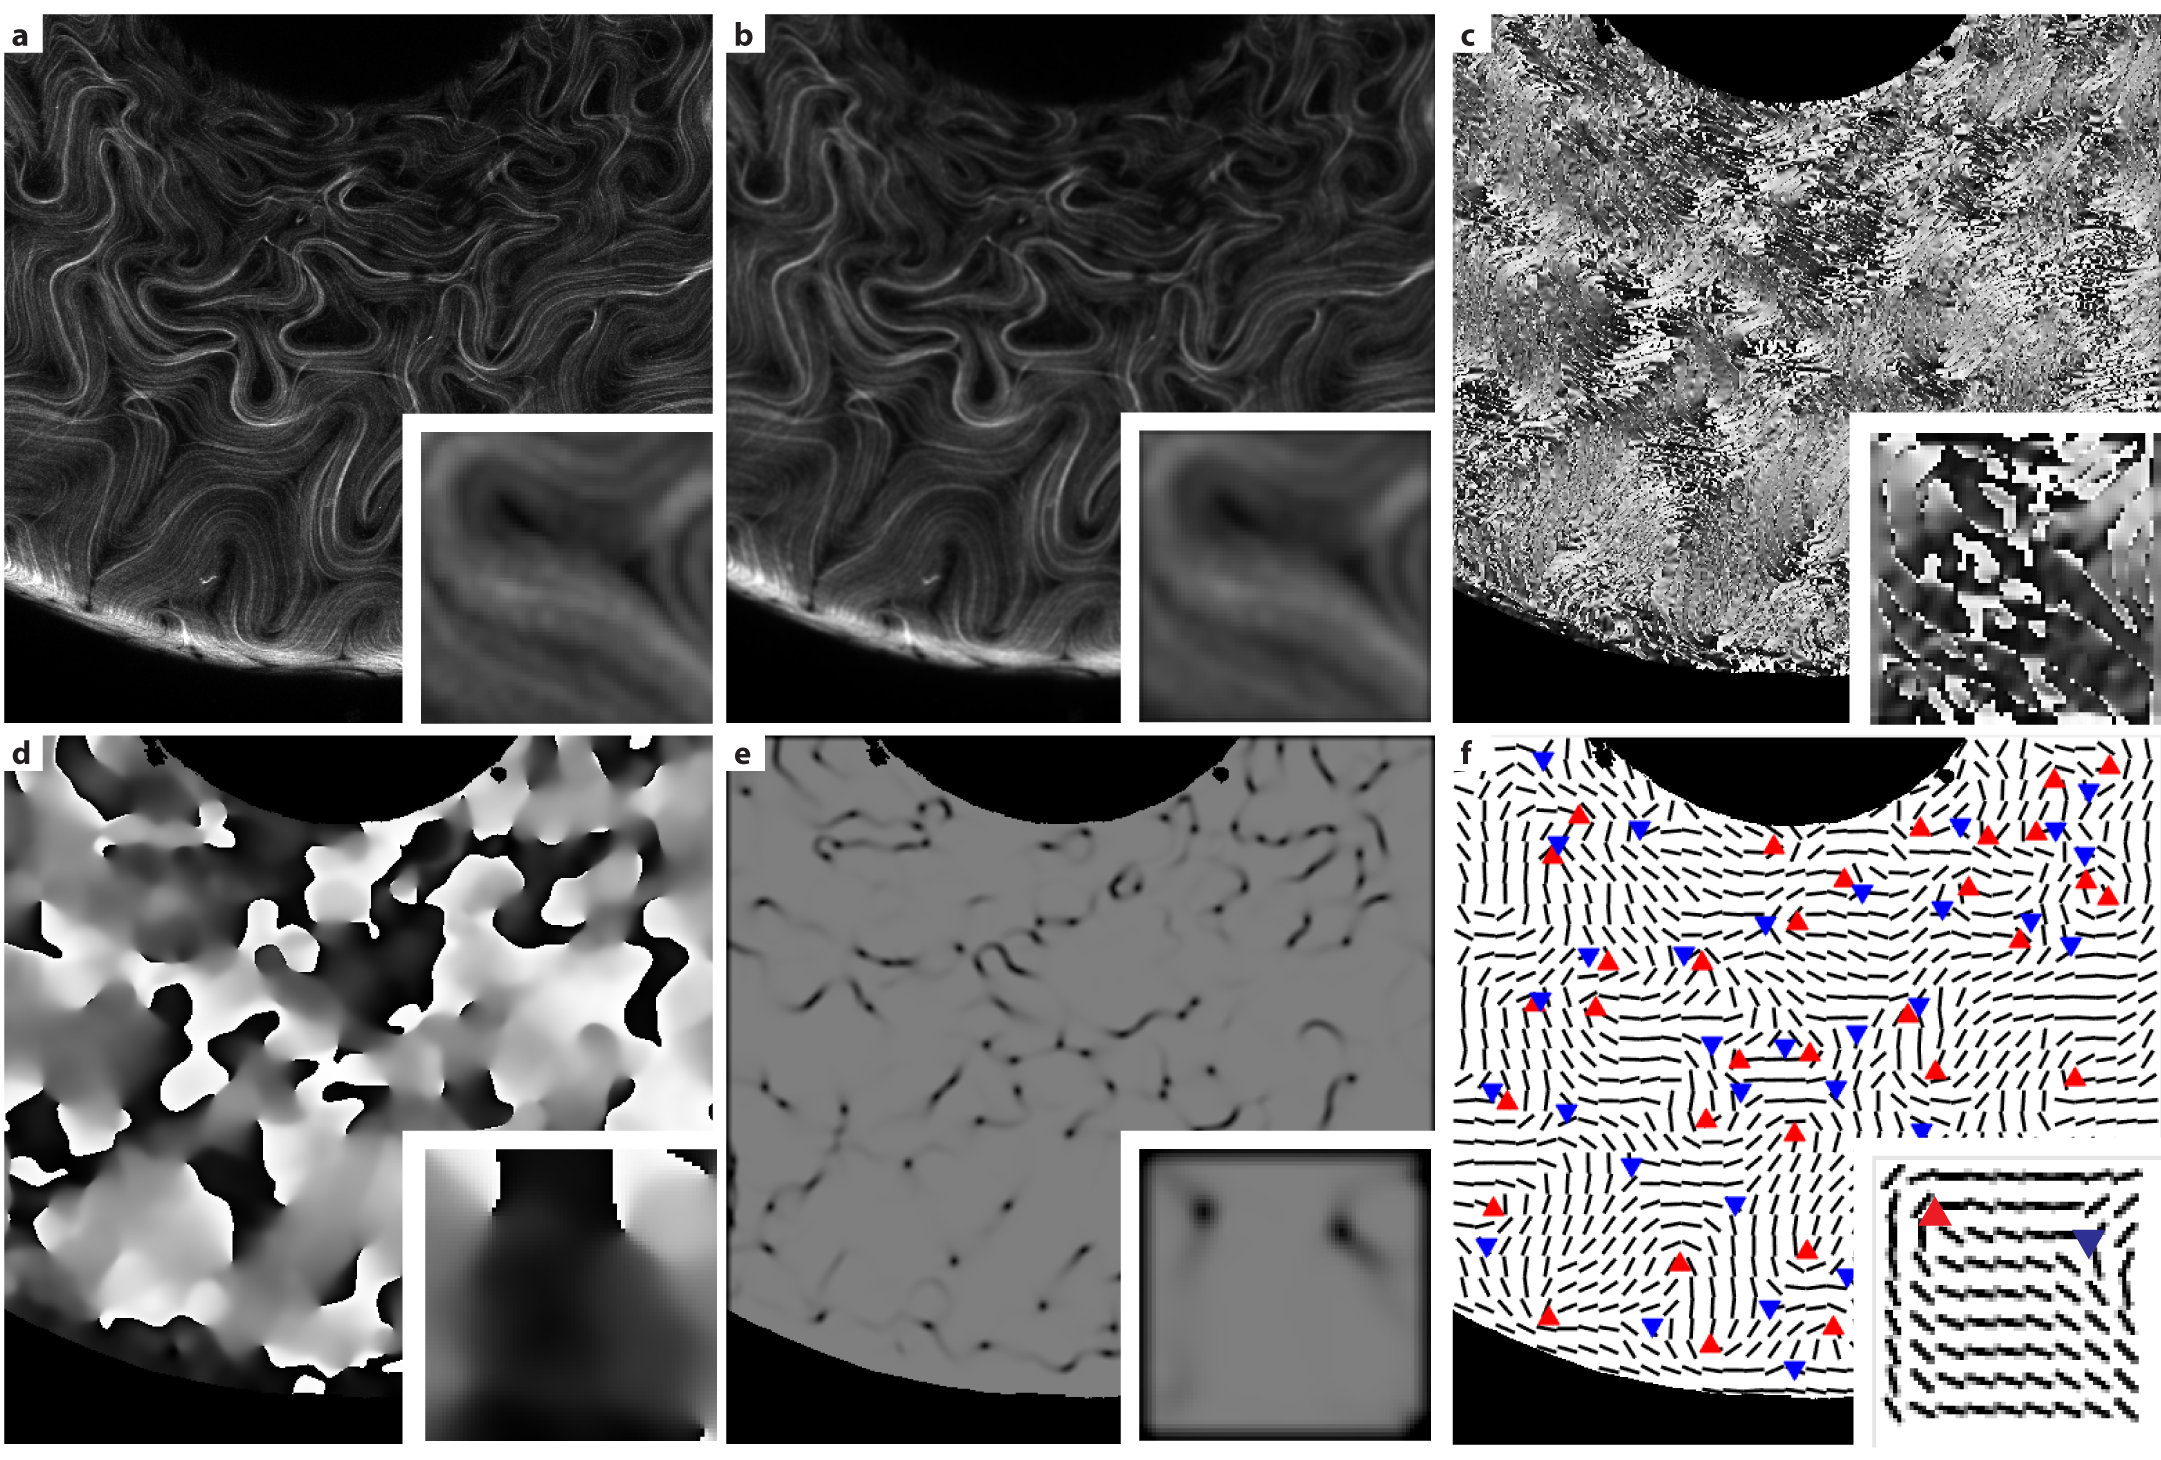
\includegraphics[width=\textwidth]{figures/C3/Ch3-Figs_CEDF2.png}
  \caption{Step-by-step output to find the director and defects from an active nematic image.
(A), Maximum-intensity projection of a confocal stack along $-\hat{z}$ at a single time.
Inset: Close up of a defect pair.
(B), Image from (A) after applying a $5 \textrm{ px} \times 5 \textrm{ px}$ Gaussian blur with standard deviation of 1 px.
Inset: The same operation applied to the image in the inset of (A).
(C), Coherence directions of the tensors formed from the gradient of the image in (B).
Black represents $0^{\circ}$ and white represents $180^{\circ}$ measured CW from the horizontal.
Inset: The same operation applied to the image in the inset of (B).
(D), Coherence directions of the structure tensors formed by component-wise averaging the gradient tensors formed from image (B).
Black represents $0^{\circ}$ and white represents $180^{\circ}$ measured CW from the horizontal.
The averaging is done with a $29 \times 29$ Gaussian filter with standard deviation of 5 px.
Inset: The same operation applied to the image in the inset of (B).
(E), The scalar order parameter $S$ obtained by diagonalizing the $\mathbf{Q}$ formed from the directions in image (D).
$\mathbf{Q}$ is formed for each point by considering the directions of all points in a 5 pixel radius.
Inset: The same operation applied to the image in the inset of (D).
(F), The director obtained by diagonalizing the $\mathbf{Q}$ formed from the direcions in image (D).
$\mathbf{Q}$ is formed for each point by considering the directions of all points in a 5 pixel radius.
The defects are calculated by considering points of low $S$ and calculating the $\mathbf{n}$-rotation along a path encircling the point.
$s = +1/2$ defects are represented by ${\color{red} \blacktriangle  } $  and $s = -1/2$ defects are represented by ${ \color{blue} \blacktriangledown  } $.
Inset: The same operation applied to the image in the inset of (D).}\label{f:3-CEDF2}
\end{figure}
\newpage
\subsection{Calculating the director}
From $\mathbf{u}$, we compute the 2D tensor nematic order parameter defined in Eq.~\ref{e:2-2DOrderRaw}, taking the average over all the $\mathbf{u}$ of all points in a specified radius of the point of interest.
We perform this averaging using a disc filter of radius $\beta$.
We then diagonalize the $\mathbf{Q}$ as shown in Eq.~\ref{e:2-2DOrderDiag}, providing $\mathbf{n}$ and $S$ for each pixel.
For the orientations of $\mathbf{u}$ in displayed in Figure~\ref{f:3-CEDF2}(D), we choose $\beta = 5$~px to produce $S$ and $n$ as shown in Figure~\ref{f:3-CEDF2}(E,F), respectively.
The greyscale intensity $[\textrm{black}, \textrm{gray})$ in Figure~\ref{f:3-CEDF2}(E) maps to the values $S = [0, 1]$ such that the dominant grey shade in Figure~\ref{f:3-CEDF2}(E) indicates uniform alignment within the 5 px radius.
In addition, note that only every $7^{\textrm{th}}$ value of $\mathbf{n}$ is plotted in Figure~\ref{f:3-CEDF2}(F) to ensure the $\mathbf{n}$-field is clear to the eye.
In reality there is a value for $\mathbf{n}$ at every pixel. \\

The process of determining the director relies on the choice of three parameters: $\sigma$, the standard deviation of the filter for the initial blur, $\rho$, the standard deviation of the filter to produce the structure tensor, and $\beta$, the radius of the disc filter used to determine $\mathbf{Q}$.
We choose the parameters such that the director field calculated on a random sampling of 3~--~5 intensity images in a given time series best agrees by eye with the actual intensity images.
We find best results keeping $\sigma = 0.5$~px and varying $\rho$ between 5~px and 8~px and varying $\beta$ between 5~px and 6~px.
The variations in $\rho$ and $\beta$ are a result of different scales between pixels and $\upmu$m depending on the microscope used, the microscope zoom, and the output image size.
However, since the initial blur is responsible for removing random noise at the pixel level, we find best results keeping $\sigma = 0.5$ px always.
Once we determine $\mathbf{n}$ and $S$, we turn to finding the defects.


\subsection{Finding defect location and topological charge}
We start by selecting pixels with $S < 0.1$ as potential defect candidates.
For every candidate, we first consider all pixels in a 5~px~$\times$~5~px plaquette centered on the point of interest and ensure that there are no other candidates in the plaquette with a lower value of $S$.
We then calculate the $\mathbf{n}$-rotation about the point of interest according to Eq.~\ref{eq:2-topCharge}.
Explicitly, we numerically evaluate $s = (1 / 2 \pi)(\oint \partial\phi / \partial u)$ CCW along the edge of the plaquette, where $u$ is the arclength parameter along the square contour and $\phi$ is the orientation of $\mathbf{n}$.
We take the point of interest to be a $s = \pm 1/2$ defect if $s \in \pm [0.49,0.51]$.
The $s=\pm1/2$ defects calculated for our example analysis are plotted on top of the $\mathbf{n}$-field in Figure~\ref{f:3-CEDF2}(F), with $s = +1/2$ defects indicated by ${\color{red} \blacktriangle } $  and $s = -1/2$ defects indicated by ${ \color{blue} \blacktriangledown } $.\\

We store the defect locations in a list recording the frame and position of each defect.
The $s = +1/2$ and $s = -1/2$ defects are stored separately.
If our time resolution is high enough, we can track the defects.
We track each species independently using a combinatorics-based particle tracking algorithm.
For tracked defects, we store the defect identity in addition to the frame and position so that we can reconstruct individual defect trajectories.\\

Due to the discrete nature of our data, it is possible to ``miss'' defects, especially when pairs of defects are close together.
Typically, since one defect in the pair will have a lower value of $S$, the defect with the larger value of $S$ will be ignored.
Since topological charge is discrete, every missed defect in a region causes the total topological charge in that region to have an error of $\pm 1/2$.
This gives us a way to characterize the error in our defect-finding routine.
We consider a region of the surface and monitor the average charge in the region over time.
We find that the time-averaged topological charge in a region converges if we average over enough time frames, implying that at least some portion of the error is random.
However, this does not exclude the presence of a systematic error such as consistently missing a single $s = -1/2$ defect --- the time-averaged charge would still converge with enough frames, but the measured value would converge to a value lower than the actual time-averaged topological charge.\\

We characterize the systematic error in the measured topological charge by considering a region of interrogation as its own entity.
Even without knowing the curvature of the surface, any region on the toroidal surface is homeomorphic to a disc with a boundary and thus according to the Guass-Bonnet theorem in Eq.~\fxnote{INTRO} has $\chi = 1$.
However, the Poincar\'e-Hopf theorem as written in Eq.~\fxnote{INTRO} only applies for surfaces with a boundary if the director at the boundary is either tangential or normal to the boundary.
In our case, the director if free to take any value on the boundary and thus can act as a source or sink of charge such that we can't write a relation between only the topological charge on the surface and the Euler characteristic of the surface.
Instead, we use an extended version of the Poincar\'e-Hopf theorem~\cite{RN267} that allows the director to vary on the boundary:
\begin{equation}
  \chi = s_{bulk} + s_{boundary} = \sum\limits_i s_i + s_{boundary},\label{e:3-extendedPH}
\end{equation}
where $s_i$ is the charge of a defect in the bulk of the region calculated via Eq.~\ref{eq:2-topCharge}, and $s_{boundary}$ is the edge charge.


\subsection{Edge charge}
Recall that the topological charge is the winding number of the director along a closed contour in $\mathbb{R}\mathbb{P}_1$, where the director is specified with respect to a fixed frame.
To find the edge charge we consider $\mathbf{n}$ along the edge and calculate the associated winding number in $\mathbb{R}\mathbb{P}_1$, but here we measure the director orientation with respect to the Frenet-Serret frame along the edge.
If we let $\phi$ describe the director orientation with respect to fixed coordinate system and $\psi$ describe the orientation of the unit tangent vector with respect to the fixed coordinate system, then $\phi' = \psi-\phi$ gives the director orientation with respect to the Frenet-Serret frame~\cite{RN35,RN23}.
Thus, we calculate the edge charge like:
\begin{equation}
  s_{boundary} = \frac{1}{2\pi} \oint \textup{d}\phi'\label{e:3-boundCharge}.
\end{equation}
Note that if we substitute the definition of $\phi'$ into Eq.~\ref{e:3-boundCharge}, we can re-write the edge charge as:
\begin{equation}
  s_{boundary} = \frac{1}{2\pi} \oint \bigg \{ \textup{d}\psi - \textup{d}\phi \bigg \} = \frac{1}{2\pi} \oint \textup{d}\psi - s_{bulk}\label{e:3-boundChargeExpand},
\end{equation}
where here $s_{bulk}$ is calculated directly due to the additivity of defects.
If we perform the integral in Eq.~\ref{e:3-boundChargeExpand} in the direction of the unit tangent vector, the Turning of Tangents theorem~\cite{RN35} lets us write $s_{boundary} = 1 - s_{bulk}$ such that for a surface with a single boundary we have $\chi = s_{bulk} + s_{boundary} = 1$.
Thus, we can determine if we have systematic error in our defect detection routine with Eq.~\ref{e:3-extendedPH}: the sum of the edge charge and the topological charge from all the defects in the bulk should be equal to one.\\

We define regions in an intensity image using a binary mask, where a $1$ means the pixel is included in the region of interest and a $0$ means the pixel is excluded.
We take the boundary of a binary mask to be the pixels with value $1$ connected by an edge to at least one $0$-valued pixel.
Along the boundary, the normalized displacement vector between two pixels indexed with $i$ and $j$ is defined as:
\begin{align}
  \Delta \mathbf{R}_{i,j} =  \frac{\mathbf{R}[j]-\mathbf{R}[i]}{|\mathbf{R}[j]-\mathbf{R}[i]|}.
\end{align}
We estimate the unit tangent vector for a pixel of interest by averaging the local normalized displacement vectors:
\begin{equation}
  \mathbf{T} \approx \frac{\Delta \mathbf{R}_{i,i+1} + \Delta \mathbf{R}_{i,i+2} + \Delta \mathbf{R}_{i-1,i} + \Delta \mathbf{R}_{i-2,i}}{|\Delta \mathbf{R}_{i,i+1} + \Delta \mathbf{R}_{i,i+2} + \Delta \mathbf{R}_{i-1,i} + \Delta \mathbf{R}_{i-2,i}|},
\end{equation}
where the pixel of interest is indexed by $i$ and an increasing index corresponds to a CCW displacement along the boundary.
To complete the Frenet-Serret frame, we estimate the outward pointing unit normal $\mathbf{k}$ by applying a $-\pi/2$ CCW rotation to $\mathbf{T}$ at every pixel.
Finally, we calculate $\phi' = \psi-\phi$ and numerically evaluate Eq.~\ref{e:3-boundCharge}.\\

The Turning of the Tangent Theorem lets us test our Frennet-Serret frame; we set $\phi = \textup{cons't}$ and find that $s_{boundary} = 1$ for our set of test masks, as desired.
We use example director fields with $s = -1, -1/2, +1/2, +1$ defects to test our full routine and confirm that $s_{boundary} + s_{bulk} = 1$ for all of our test cases.\\


We now consider a region in the intensity projection for a torus and monitor the average $s_{bulk}$ and $s_{boundary}$ over time, where we calculate $s_{bulk} = \sum\limits_i s_i$, with $s_i$ the charge of a single defect in the bulk of the region.
We find that even though there is approximately a $50\%$ chance of missing a defect in the region, the error is random and not systematic such that $\overbar{s}_{bulk} + \overbar{s}_{boundary} = 1$ if we average for enough frames.





\section{Measuring surface curvature}
From $h(x,y)$, we wish the calculate the Gaussian curvature of the surface.
Recall from Chapter~\ref{c:1} that $K = \textup{det} \big \{ \mathbf{L} \big \}$.
Thus, we need to calculate the Weingarten matrix, defined as $\tensor{L}{_j^i} = -(\nabla_j \mathbf{k}) \cdot \mathbf{e}^i$, where $\mathbf{k}$ is the unit surface normal and $\mathbf{e}^i = g^{ij}(d \mathbf{R}/dx^j)$ is the basis covector in the $i^{\textrm{th}}$ direction~\cite{RN35}.


\subsection{The Weingarten matrix}
Since $\mathbf{R} = \{x, y, h(x,y)\}$, it is straightforward to calculate the Weingarten matrix directly.
However, this involves taking discrete first and second derivatives on a noisy surface.
To avoid this, we notice that the Weingarten matrix relates a displacement in the tangent plane of a surface with the corresponding change in the unit normal vector along the displacement like:
\begin{equation}
\nabla_j \mathbf{k} \cdot \Delta \mathbf{r} = -\tensor{L}{_j^i} \mathbf{e}_i \cdot \Delta \mathbf{r},\label{e:3-Kfit1}
\end{equation}
with $\mathbf{\Delta r} = \Delta r^j \mathbf{e}_j$ an arbitrary displacement in the tangent plane.
Note that the relation $\nabla_j \mathbf{k} = -\tensor{L}{_j^i} \mathbf{e}_i$ is called Weingarten's formula and comes from the fact that the change in the surface normal due to infinitesimal displacements in the tangent plane exists solely in the tangent plane~\cite{RN35}.
Thus, for a point of interest on the surface, we can consider local displacement vectors and the corresponding change in the unit surface normal and then fit $\tensor{L}{_j^i}$ according to Eq.~\ref{e:3-Kfit1} using an iteratively-reweighted least squares (IRLS) routine~\cite{RN32,RN31}.
This technique allows us to characterize a noisy surface without taking a discrete derivative and without any prior knowledge about the surface features.
In addition, an IRLS routine is a robust fit able to reject outliers and accommodate the noise in our data.


\subsection{Iteratively-reweighted least squares}
Consider a set of observations of an independent dependent random variable where each observation is denoted by $y_i$ and is associated with a dependent variable $x_i$.
Given a model $y'_i = g(x_i,\bm{\alpha})$, where $\bm{\alpha}$ is the parameter vector for the model, we can define the error of the model for each observation by the residual, $\gamma_i = y_i - y'_i = y_i - g(x_i,\bm{\alpha})$.
A least-squares fit works to find the $\bm{\alpha}$ that minimizes the sum of the squared residuals:
\begin{equation}
  \argmin_{\bm{\alpha}} \sum\limits_i\, \big \{ \gamma_i^2\big \}.\label{e:3-LeastSquare}
\end{equation}
If the model is linear, the fit has an analytic solution~\cite{RN269}.
In addition, for normally-distributed data, the result of least squares fit gives the maximum-likelihood values of $\bm{\alpha}$~\cite{RN269}.
This is illustrated in Figure~\fxnote{fits}(A), where $x_i$ and $y_i$ are linearly related such that a line fits the example data well and $\bm{\alpha}$ contains the slope and the intercept of the line.\\

However, least-squares fits are very sensitive to outliers in the data and thus do not do well when the data are very noisy.
This is easy to see in Figure~\fxnote{fits}(B), where we introduce some outliers into our example data from Figure~\fxnote{fits}(A).
The fact that Eq.~\ref{e:3-LeastSquare} tries to minimize the sum of the squared errors means that outliers can have a disproportionate effect on the final fit.
In fact, extreme outliers are often referred to as lever points for this exact reason.\\

One way to treat noisy or uncertain data is to assign a weight to each data point such that data points with larger error are weighted less.
The fit then becomes:
\begin{equation}
  \argmin_{\bm{\alpha}} \sum\limits_i\,\big \{ (w_i \gamma_i)^2 \big \},
\end{equation}
where $w_i$ is the weight associated to the observation $y_i$.
A weighted linear least-squares fit of this type is still analytically solvable~\cite{RN269}.
Unfortunately, weighted least-squares is still very sensitive to outliers if it is not obvious \emph{a priori} which data are the outliers. \\

One way to deal with this is to construct a fit that is inherently less sensitive to outliers.
For example, we can replace the square of the residual with a general cost function:
\begin{equation}
  \argmin_{\bm{\alpha}} \sum\limits_i\,\textrm{cost}(\gamma_i),\label{e:3-GeneralCostFit}
\end{equation}
such that the fit could deprioritize or even reject entirely large sources of error.
These cost functions are known as maximum-likelihood-type estimators, or M-estimators~\cite{RN269}.
Note that choosing the cost function $\textrm{cost}(\gamma_i) = \gamma_i^2$ gives a regular least-squares fit.
Unfortunately, a general cost function is not often analytically solvable or easy to minimize.
However, provided the cost function is differentiable, we can solve Eq.~\ref{e:3-GeneralCostFit} with an IRLS process.\\

We begin by expressing Eq.~\ref{e:3-GeneralCostFit} in terms of a weighted least-squares fit.
Taking the derivative of Eq.~\ref{e:3-GeneralCostFit} with respect to $\bm{\alpha}$ gives:
\begin{equation}
  \sum\limits_i\,\frac{\partial \, \textrm{cost}(\gamma_i)}{\partial \gamma_i} \frac{\partial \gamma_i}{\partial \bm{\alpha}} = 0.\label{e:3-IRLSderiv1}
\end{equation}
If we define a weight function like $w(\gamma_i) = \dfrac{1}{\gamma_i}\dfrac{\partial \, \textrm{cost}(\gamma_i)}{\partial \gamma_i}$, we can now re-write Eq.~\ref{e:3-IRLSderiv1} as:
\begin{equation}
  \sum\limits_i\,w(\gamma_i) \gamma_i \frac{\partial \gamma_i}{\partial \bm{\alpha}} = 0.\label{e:3-IRLSderiv2}
\end{equation}
 Solving Eq.~\ref{e:3-IRLSderiv2} for $\bm{\alpha}$ is equivalent to minimizing:
 \begin{equation}
   \argmin_{\bm{\alpha}} \sum\limits_i\,\big \{ (w_i(\gamma_i) \gamma_i(\bm{\alpha}))^2 \big \},\label{e:3-WeightLS}
 \end{equation}
a weighted least-squares fit, where we have expressed $\gamma_i$ inside the minimization as an explicit function of $\bm{\alpha}$ for clarity.
However, since our weights are dependent on the residuals, we solve Eq.~\ref{e:3-WeightLS} iteratively, where the weights for an iteration $(p)$ are determined by the residuals from the previous iteration, giving:
\begin{equation}
  \bm{\alpha}^{(p+1)} = \argmin_{\bm{\alpha}} \sum\limits_i\,\bigg \{ \bigg [w_i \big(\gamma_i^{(p)}\big ) \gamma_i(\bm{\alpha}) \bigg ]^2 \bigg \}.
\end{equation}
With enough iterations, the $\gamma_i$ converge and we have the $\bm{\alpha}$ values that solve Eq.~\ref{e:3-WeightLS}.
The entire process can described by the recursion relation:
\begin{equation}
  \gamma_i^{(p+1)} = y_i - g\big (x_i,\bm{\alpha}^{(p+1)}\big )= y_i - g\Bigg (x_i, \argmin_{\bm{\alpha}} \sum\limits_i\,\bigg \{ \bigg [w_i \big(\gamma_i^{(p)}\big ) \gamma_i(\bm{\alpha}) \bigg ]^2 \bigg \} \Bigg).
\end{equation}

Since these cost functions do not need to be everywhere convex, they may not necessarily have a global minimum, or even a guaranteed convergence.
However, those that are not globally convex often deal with large error more severely than convex functions.
Thus, to get the best of both worlds, we will first fit our surface using the convex ``Fair'' M-estimator~\fxnote{Fair citation} until the fit converges, then fit the output of the Fair fit with the non-convex ``Geman-McClure'' (GMC) M-estimator~\cite{RN52}.
The functional forms and weight functions of some common M-estimators as well as the twq M-estimators we use are found in Table~\ref{t:3-CostFxn} and plotted in Figure~\ref{f:3-CostFxn}.
\newpage
\begin{table}[ht]
  \centering
  \caption{Cost and weight functions of common M-estimators.\@$x$ are the residuals and $c$ is a tuning parameter.}
  \begin{tabular}{|r c c |}
    \hline \\[-0.45cm]
     & $\textrm{cost}(x)$ & $w(x)$\\
    \hline \\[-0.3cm]
    {\bf least-squares}:& $\dfrac{x^2}{2}$ & 1\\ [0.5cm]
    {\bf L$_p$}:& $ \dfrac{|x|^p}{p} $ & $|x|^{p-2}$\\[0.5cm]
    {\bf Fair}:& $c^2 \Bigg [ \dfrac{|x|}{c} - \log \Big ( 1 + \dfrac{|x|}{c}\Big ) \Bigg ]$ & $\dfrac{1}{1 + |x|/c}$ \\ [0.5cm]
    {\bf Geman-McClure}:& $\dfrac{(x/c)^2}{1+(x/c)^2}$ & $\dfrac{2}{(1+(x/c)^2)^2}$ \\ [0.5cm]
    {\bf Cauchy}:& $\dfrac{c^2}{2} \log \big ( 1 + (x/c)^2 \big)$ & $\dfrac{1}{1 + (x/c)^2}$\\ [0.5cm]
    \hline
  \end{tabular}\label{t:3-CostFxn}
\end{table}

\begin{figure}[hb]
  \centering
  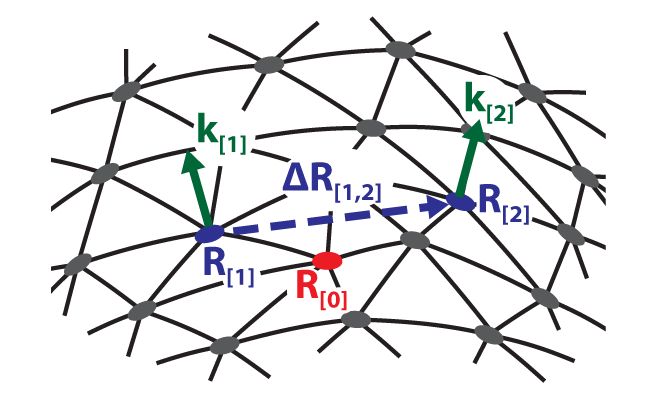
\includegraphics{figures/C3/Ch3-Figs_CurvFitSchem.png}
  \caption{Plots of the cost functions and weight functions for common M-estimators.}\label{f:3-CostFxn}
\end{figure}
\newpage
\subsection{Fitting the Weingarten matrix on a surface}
From a Monge parameterization $h(x,y)$ of a surface~\cite{RN35,RN23}, we start by computing the Delauney triangulation~\cite{RN34} such that every point in $h(x,y)$ is a vertex in the triangulation.
From the triangulation, we estimate $\mathbf{k}$ at every vertex as the average of the unit normals of the adjacent faces.
Once we have a triangulation and the $\mathbf{k}$ estimates, we proceed to fit the curvature.\\

Let $\mathbf{R}_0$ be an example point of interest with normal $\mathbf{k}_0$.
We first make an initial fit using regular least-squares to serve as an input into the IRLS routine.
We consider all points within $d_1$ of $\mathbf{R}_0$ to be within the region of interest and then use $\mathbf{k}_0$ to transform the region of interest into the tangent plane of $\mathbf{R}_0$.
We then calculate $\Delta \mathbf{R}_{ij} = \mathbf{R}[j]-\mathbf{R}[i]$ and $\Delta \mathbf{k}_{ij} = \mathbf{k}[j]-\mathbf{k}[i]$ for every possible pair of points in the region of interest, with individual points indexed with $i$ and $j$, $\mathbf{R}_0 = \mathbf{R}[0]$, and $\mathbf{k}_0 = \mathbf{k}[0]$ .
Importantly, the pairs of points do note need to include the $\mathbf{R}_0$; this reduces the influence of error in $\mathbf{R}_0$ and $\mathbf{k}_0$.
Since the Weingarten matrix only considers variations in $\mathbf{k}$ in the tangent plane, we will fit instead to an extended Weingarten matrix $\bm{\Lambda}$~\cite{RN31,RN32}:
\begin{equation}
\begin{pmatrix}
\Delta \mathbf{k} \cdot \bm{e}_1 \\
\Delta \mathbf{k} \cdot \bm{e}_2 \\
\Delta \mathbf{k} \cdot \mathbf{k}_0
\end{pmatrix}
=
\begin{pmatrix}
\tensor{L}{_1^1} & \tensor{L}{_1^2} \\
\tensor{L}{_2^1} & \tensor{L}{_2^2} \\
M_{1} & M_{2}
\end{pmatrix}
\begin{pmatrix}
\Delta \bm{R} \cdot \bm{e}_1 \\
\Delta \bm{R} \cdot \bm{e}_2
\end{pmatrix},
\label{e:3-Kfit2}
\end{equation}
where we have added $M_1$ and $M_2$ to $\mathbf{L}$ to form $\bm{\Lambda}$.
This additional information will eventually allow us to re-estimate $\mathbf{k}$~\cite{RN31}. \\

We now have a system of three equations to fit with 5 parameters, as $\tensor{L}{_1^2} = \tensor{L}{_2^1}$.
If we naively expand Eq.~\ref{e:3-Kfit2} directly into three equations,
\refstepcounter{equation}\label{e:3-KfitNaive}
\begin{align}
  \Delta k_1 &= \tensor{L}{_1^1} \Delta R_1 + \tensor{L}{_1^2} \Delta R_2\tag{\theequation a} \\
  \Delta k_2 &= \tensor{L}{_2^1} \Delta R_1 + \tensor{L}{_2^2} \Delta R_2\tag{\theequation b} \\
  \Delta k_k &= M_1 \Delta R_1 + M_2 \Delta R_2,\tag{\theequation c}
\end{align}
where we have expanded the vectors like $\mathbf{v}\cdot \mathbf{e}_i = v^j g_{ij} = v_i$ and $\Delta k_k$ refers to the component of $\Delta \mathbf{k}$ along the surface normal, we see that $\tensor{L}{_1^2}$ will be determined entirely by the variation along $\mathbf{e}_2$.
The result of $\tensor{L}{_1^2}$ from fitting Eq.~\ref{e:3-KfitNaive}a will then set the value of $\tensor{L}{_2^1}$ in the fit of Eq.~\ref{e:3-KfitNaive}b so that only $\tensor{L}{_2^2}$ is free to vary during the fit.
This means that in principle, the choice of $\mathbf{e}_i$ could affect the output curvature.
To account for this, we rearrange Eq.~\ref{e:3-KfitNaive} to be:
\refstepcounter{equation}\label{e:3-KfitConstrained}
\begin{align}
  \Delta k_2 \Delta R_2 - \Delta k_1 \Delta R_1 &= (\Delta R_2)^2 \tensor{L}{_2^2} - (\Delta R_1)^2 \tensor{L}{_1^1}\tag{\theequation a}\\
  \Delta k_1 + \Delta k_2 - \tensor{L}{_1^1} \Delta R_1 - \tensor{L}{_2^2} \Delta R_2 &= (\Delta R_1 + \Delta R_2)\tensor{L}{_1^2}\tag{\theequation b}\\
  \Delta k_k &= M_1 \Delta R_1 + M_2 \Delta R_2.\tag{\theequation c}
\end{align}
If we do the fits in order, the values of $\tensor{L}{_1^1}$ and $\tensor{L}{_2^2}$ from fitting Eq.~\ref{e:3-KfitConstrained}a are inserted as fixed parameters into the fit of Eq.~\ref{e:3-KfitConstrained}b.
However, now the value of $\tensor{L}{_1^2}$ is determined by the variation in both directions in the tangent plane.
Once we have estimates of the elements of $\bm{\Lambda}$ from the initial least-squares fit, we move on to fitting the curvature with the IRLS routine. \\

We now choose all points within $d_2$ of $\mathbf{R}_0$, where $d_2 > d_1$, and as before, transform into the tangent plane and calculate the associated $\mathbf{\Delta N}_{ij}$ and $\mathbf{\Delta r}_{ij}$ between all pairs of points.
In addition, we calculate a geometric weight for each $\mathbf{\Delta r}_{ij}$:
\begin{equation}
  m_{ij} = \frac{\textrm{C}} {(\mathbf{R}[i] - \mathbf{R}_0)^2 + (\mathbf{R}[j]-\mathbf{R}_0)^2},
\end{equation}
where $\textrm{C}$ is a normalization constant.
The geometric weight ensures that data far from $\mathbf{R}_0$ contribute less to the curvature at $\mathbf{R}_0$~\cite{RN32,RN31}.
We then pass the $\mathbf{\Delta N}_{ij}$, the $\mathbf{\Delta r}_{ij}$, the $m_{ij}$, the initial values in $\bm{\Lambda}$, the appropriate tuning parameters, and a convergence tolerance to our IRLS routine.
Our routine starts by calculating the residuals using $\bm{\Lambda}$ from previous fit like:
\begin{equation}
  \gamma_{ij}^{(p)} = \sqrt{(\mathbf{\Delta N}_{ij}- \mathbf{\Lambda}^{(p)} \mathbf{\Delta r}_{ij})^2},
\end{equation}
where $p$ is the iteration number and the $0^{\textrm{th}}$ iteration refers to the initial least-squares fit.
The routine then calculates the weights for the Fair M-estimator seen in Table~\ref{t:3-CostFxn}, multiplies the Fair weights for each pair of points with the associated $m_{ij}$ to get the final fitting weight, performs a weighted least-squares fit of Eqs.~\ref{e:3-KfitConstrained}, and then repeats the process from the beginning until the fit converges.
For the fair fit we take the tuning constant $c_F^{(p+1)} = c_F^{initial} \, \textrm{median}\{ \bm{\gamma}^{(p)} \}$, where $p$ is the iteration number, $c_F = 1.3998$ corresponds to 95\% efficiency on a standard normal distribution, $\bm{\gamma}^{(p)}$ is a vector of the residuals, and $c_F^{initial}$ is an input parameter.
Efficiency refers to how much data an M-estimator needs to get the maximum likelihood solution.
A true least-squares fit has 100\% efficiency --- as data are included in the fit, a least-squared fit approaches the true values of the parameters the ``fastest,'' hence the fact that a least squares fit is 100\% efficient~\cite{RN269}.
We include the median of the residuals in our tuning constant so that the tuning parameter in the fit doesn't need to be adjusted as much between datasets with different levels of noise.
In addition, we ensure that the $c_F^{(p)} \leq c_F^{(0)}$.
The Fair fit converges when the cost function changes by less than the specified convergence tolerance between subsequent iterations.
While we set an upper limit of 50 iterations for the Fair fit, the fit typically converges in fewer than 20 iterations taking the convergence tolerance to be 0.001.\\

The final values of $\bm{\Lambda}$ from the Fair fit are then used as the initial values for an IRLS fit using a GMC M-estimator.
The overall flow of the algorithm is the same for the GMC M-estimator as it was for the Fair M-estimator.
However, there are some key differences in how the fitting weights are handled.
Here, we include the possibility to reject outliers by calculating the fitting weights as:
\begin{equation}
  w_{ij}^{(p+1)} =
\begin{cases}
0, & \text{if} \quad \gamma_{ij}^{(p)} > b \ c_{GMC}^{(p)} \\
 \dfrac{2}{(1+(\gamma_{ij}^{(p)} / c_{GMC}^{(p)})^2)^2}, & \text{otherwise}
\end{cases},
\end{equation}
where $c_{GMC}^{(p)} = c_{GMC}^{initial} \, \textrm{median}\{ \bm{\gamma}^{(p)} \}$ is the tuning constant for the GMC fit, $c_{GMC}^{initial}$ and $b$ are an input parameters, and $c_{GMC} = 1.4826$ corresponds to 95\% efficiency on the standard normal distribution.
Here we have modified the standard GMC weight function to exclude data whose residual is too large.
The outlier rejection works fundamentally by comparing each residual against the median residual.
The parameter $b$ then determines how much variance with respect to the median residual is allowed.
As with the Fair fit, we ensure that the $c_{GMC}^{(p)} \leq c_{GMC}^{(0)}$.
The GMC fit converges when the cost function changes by less than the specified convergence tolerance between subsequent iterations.
We set an upper limit of 20 iterations for the GMC fit, but the fit typically converges in fewer than 10 iterations when taking the convergence tolerance to be 0.001. \\

The routine outputs the GMC weights from the final fitting iteration and the final values of $\bm{\Lambda}$.
Finally, we calculate the mean and Gaussian curvature of at $\mathbf{R}_0$ taking $H = \textup{Tr}\{ \mathbf{L} \}/2$ and $K = \textup{det}\{ \mathbf{L} \}$ and move on to correcting $\mathbf{k}_0$.


\subsection{Correcting the surface normal vectors}
We use the fitting weights from the final iteration $(p)$ and the final values in $\bm{\Lambda}$ to correct our initial estimate of $\mathbf{k}_0$ using a weighted average~\cite{RN31}:
\begin{equation}
\mathbf{k}_0^{(p)} = \frac{\sum\limits_i m_{0i}w_{0i}^{(p)}(\mathbf{N}_i^{(0)} - \mathbf{\Lambda}^{(p)}\mathbf{\Delta R}_{0i})}{\sum\limits_j m_{0j}w_{0j}^{(p)}},.
\end{equation}
where $\mathbf{k}_0^{(p)}$ corresponds to the re-estimated unit normal.
Note that here we have only used pairs of points that include $\mathbf{R}_0$.
This re-estimation uses the fitted curvature to determine what the surface normal should be.
We now transform $\mathbf{k}_0^{(p)}$ back into the original coordinate system, and then repeat the entire fitting process for another point on the surface.


\subsection{Finding the area element}
Once we have the re-estimated normal vectors everywhere on the surface, we can calculate the determinant of the metric~\cite{RN35},
\begin{equation}
g = \frac{1}{(\mathbf{k}_0^{(p)} \cdot \mathbf{\hat{z}})^2}.
\end{equation}
The determinant of the metric lets us connect areas in our flat intensity projection with areas on our curved toroidal surface via the local area element~\cite{RN35}, $\textrm{dA} = \sqrt{g} \, \textrm{dx}\textrm{dy}$.
Physically, we see that in the Monge parameterization, $\sqrt{g}$ reflects the tilt angle of the surface when compared to the flat plane that parameterizes the height of the surface.


\subsection{Validation on test surfaces}
We validate our routine on hemispheres and saddle-like surfaces with varying levels of random noise inserted into the height of the surface in order to mimic the noise in our confocal data.
We specify the noise as a percentage of the radii of curvature used to generate the test surface.
Surfaces with less than 1\% noise or no noise are overall insensitive to $d_1$, $d_2$, and the tuning constants in the fit.
We test surfaces with up to 3\% noise and find that setting $b=2$ and $c_{F}^{inital}$ and $c_{GMC}^{inital}$ to their respective 95\% efficiency values works well.
In addition, we see that $d_2$ matters far more than $d_1$, increasing $d_2$ improves the noise tolerance of the fit.
For a given amount of noise, we fit a test surface multiple times while increasing $d_2$ until the change in the curvature with increasing $d_2$ is small enough.
While we could in principle set $d_2$ to the size of the surface, our fit scales factorially with increasing $d_2$ such that we must balance runtime against improvements in the output curvature.
We find that setting $d_2 > 12$ yields impractical runtimes.\\

Overall, our curvature fitting routine works well far from the boundaries.
Near the boundaries, the curvature fit does not always work very well as there is less long-range information availible when a point is within $d_2$ of a boundary.
As a consequence, we typically neglect curvature values within $d_2/2$ of the boundary.


\subsection{Measuring the curvature of toroidal droplets}
Before we measure the curvature of the $h(x,y)$ output from time-averaging the intensity of a confocal image stack, we first have to remove measurement artifacts.
Since $h(x,y)$ is discrete quantity set by the height resolution of the confocal, the measured surface appears to have ``steps'' where the measured surface jumps from the height of one image plane to another.
Fitting the curvature on such a surface with reasonable $d_2$ values would yield large areas with vanishing $K$ between steps interspersed with areas with large $|K|$ near each step.
We remove the steps by downsampling the initial $h(x,y)$ until the output triangulation just appears smooth.
If we downsample too much, we risk eliminating real curvature features in our data.
In practice, we typically downsample $h(x,y)$ with an initial size 512~px~$\times$~512~px to a final size 75~px~$\times$~75~px.
We fit the curvature on the downsampled $h(x,y)$ with $d_1 = 4$ and $d_2 = 12$, and then upsample the final $K(x,y)$, $H(x,y)$, and $\sqrt{g}(x,y)$ back to the original size using linear interpolation.




\section{Defect charge and curvature}
From the fitted curvatures and the defect locations over time, we look to compare the time-averaged topological charge in a region with the integrated Gaussian curvature of the region.


\subsection{Finding regions of specific integrated Gaussian curvature}
We start by considering a binary mask where the region in the intensity projection where we have data for the director field has a value $1$ and everywhere else has a value $0$.
We then remove the outer 10~px to 30~px of the region by successively finding the boundary of the region and setting the boundary to $0$ until the mask only indicates places where we trust the curvature.
This mask serves as our base from which we will determine any region we with to look at.
For any mask $\Theta(x,y)$ defining a region, we calculate the integrated Gaussian curvature numerically,
\begin{equation}
  \oint_{\Theta}\,K\textrm{dA} \approx \sum\limits_{x,y} \Theta(x,y) K(x,y). \sqrt{g}(x,y)
\end{equation}
Since the area is positive-definite, the maximum integrated Gaussian curvature and the minimum integrated Gaussian curvature masks are easy to generate simply by starting with the base mask and setting the pixels with $K < 0$ or $K > 0$ to $0$.
These two masks define the range of integrated Gaussian curvature that we can probe for a single toroid.
We can also easily divide the base mask into halves or thirds to consider regions of different integrated Gaussian curvature.
However, in all of these cases the mask is determined before the integrated Gaussian curvature is calculated, leading to gaps in the integrated Gaussian curvature data. \\

We remedy this with a routine to find masks corresponding to specific values of integrated Gaussian curvature.
From a starting mask we calculate the starting integrated Gaussian curvature and determine whether it is greater or less than the desired value.
The routine then finds the boundary of the region and sets the all the pixels on the boundary with the appropriate signed $K$ to $0$.
For example, if the current value if greater than the target value all the boundary pixels with $K > 0$ are set to $0$.
This process is repeated until the difference between the current value and the target value changes sign.
The routine then takes the most recently removed boundary pixels and adds them back to the mask one-by-one until the difference between the current value and the target value has the same sign as the difference between the initial value and the target value.


\subsection{Measuring defect charge in a specified region}
For each point in time, we create a pair of binary masks to hold the defect locations, giving the final binary arrays $J^{(+)}(x,y,t)$ and $J^{(-)}(x,y,t)$ holding the $s = +1/2$ and $s = -1/2$ defects, respectively.
Defect locations in $J$ are represented by a $1$ with all other pixels set to $0$.
Thus, we can determine the number of $s = +1/2$ and $s = -1/2$ defects in a region denoted by $\Theta(x,y)$ over time $N^{(\pm)}_{\Theta}(t)$ with the sum $N^{(\pm)}_{\Theta}(t) = \sum\limits_{xy}\,J^{(\pm)}(x,y,t)\Theta(x,y)$.
With $\overbar{N}^{(\pm)}_{\Theta} = (1/T)\sum\limits_t \, N^{(\pm)}_{\Theta}(t)$ we calculate the time-averaged topological charge in a region as $\overbar{s}_{\Theta} = (\overbar{N}^{(+)}_{\Theta} - \overbar{N}^{(-)}_{\Theta})/2$.


\subsection{Time-averaged defect charge as a function of integrated Gaussian curvature: defect unbinding}
We correlate the time-averaged topological charge in a region with the integrated Gaussian curvature of that region for both 36~mM ATP and 144~mM ATP.
We find that for both ATP concentrations, $\overbar{s}_{\Theta}$ is linear with $\oint_{\Theta}\,K\textrm{dA}$, a shown in Fig.~\fxnote{Fig}, where we plot data from toroids with a range of $\xi$ and $a$.
The slope of the curve, $C'$, is positive, consistent with the curvature-induced defect unbinding predicted theoretically.
However, due to the large number of defects and their motion, the time-averaged topological charge approaches a continuous distribution.
Furthermore, $\overbar{s}_{\Theta}$ only depends on the integrated Gaussian curvature and is independent of $\xi$ and $a$.
This implies that the unbinding only depends only on the local geometry and is insensitive to the  global size and shape of the system.
Note that this is direct contrast to equilibrium simulations and theory, which all predict dependence on $\xi$ and $a$~\cite{RN36,RN19,RN22,RN20,RN78}.
We also note that the line in Fig.~\fxnote{Fig} goes through 0, indicating that regions with $\oint_{\Theta}\,K\textrm{dA} = 0$ have $\overbar{s}_{\Theta} = 0$, a topological requirement for the entire toroid.
In our case, however, we see that this is true irrespective of the region we consider, provided the region has vanishing integrated Gaussian curvature.
This implies that a region with $\oint_{\Theta}\,K\textrm{dA} = 0$ is representative of entire toroid.
Again, this is in contrast to equilibrium nematics, where the small defect number and lack of significant defect motion result in different regions with the same net integrated Gaussian curvature generally enclosing a different topological charge.
Finally, we see that changing the ATP concentration yields a different amount of unbinding, with a lower ATP concentration unbinding more than a higher ATP concentration. \\

Thus, our results suggest that activity is playing a role akin to temperature in equilibrium systems.
In 2D, the  nematic-isotropic phase transition is predicted to be continuous~\cite{RN172}, such that the nematic elasticity should vanish smoothly on the approach to the phase transition.
As an equilibrium nematic gets sufficiently close to the nematic-isotropic, thermal fluctuations will dominate the vanishing elasticity, mobilizing the defects and producing results qualitatively similar to adding activity to the nematic.




\section{Defect number and curvature}
We also consider the relation between the defect number density and the curvature of the surface.


\subsection{Time-averaged defect density}
Here, we correlate the time-averaged defect density in a region  $\overbar{N}^{(\pm)}_{\Theta}/A_{\Theta}$ with the mean Gaussian curvature in the region:
\begin{equation}
  \langle K \rangle_{\Theta} = \frac{\int_{\Theta}K\textrm{dA}}{A_{\Theta}},
\end{equation}
where $A_{\Theta} = \int_{\Theta}\, \textrm{dA} \approx = \sum\limits_{xy}\Theta(x,y)\sqrt{g}(x,y)$ is the area of the region of interest.
We start by just considering the same regions we used to investigate the relation between integrated Gaussian curvature and time-averaged topological charge.
Like the topological charge and integrated Gaussian curvature, we see that the time-averaged defect density for both defect species varies linearly with mean Gaussian curvature, with the slope of the relation between $\overbar{N}^{(\pm)}_{\Theta}/A_{\Theta}$ and $\langle K \rangle_{\Theta}$ given by $C^{(\pm)}$.
However, we see that $C^{(\pm)}$ seems to depend on aspect ratio for a 36~$\upmu$M ATP concentration, even though the difference $(C^{(+)} - C^{(-)}) \sim C'$ does not.
In addition, we see that generally, $C^{(\pm)} < 0$ regardless of ATP concentration.
This means that the defect density is higher in regions of negative Gaussian curvature. \\

Since regions with vanishing integrated Gaussian curvature are representative of the full torus, we take the total defect number density $\overbar{N}_{\Theta}/A_{\Theta} = \overbar{N}^{(+)}_{\Theta} + \overbar{N}^{(-)}_{\Theta}/A_{\Theta}$ in regions with $\langle K \rangle_{\Theta} = 0 $ to be the defect number density of the entire toroid.
For each toroid, this quantity is the intercept of the relation between $\overbar{N}_{\Theta}/A_{\Theta}$ and $\langle K \rangle_{\Theta}$.
We see that higher ATP concentrations result in higher defect densities, consistent with previous experiments. \\

Note that the maximum and minimum $\langle K \rangle_{\Theta}$ values are not given by the regions with maximum and minimum integrated Gaussian curvature.
To see how the defect density behaves over the entire $\langle K \rangle_{\Theta}$ range, we bin the surface in $K$.
We set the binsize as a percentage of $M$, the total number of pixels with value $1$ in the base mask, such that the bins have the same number of pixels but different areas on the surface of the torus.
The first bin contains the $M'$ pixels with the smallest $K$.
We then form the remaining bins one at a time by removing the pixel in $M'$ with the smallest $K$ and then adding to $M'$ the pixel with the smallest $K$ that has never been in $M'$.
Thus, the bins overlap as much as possible and there are $M-M'+1$ bins.
When we plot $\overbar{N}_{\Theta}/A_{\Theta}$ vs $\langle K \rangle_{\Theta}$ using this protocol, we see that the linear relationship between $\overbar{N}_{\Theta}/A_{\Theta}$ and $\langle K \rangle_{\Theta}$ does not persist over the entire surface, but only for a portion of the central region.


\subsection{Defect number distributions}
Because of the constant creation and annihilation and mobility of the defects, the defect number in a region fluctuates over time.
For the 144~$\upmu$M ATP toroids, we have enough timeframes to characterize the fluctuations with the defect number distribution.
We see that the defect number distribution in Gaussian, as shown in Figs.~\fxnote{Fig} for a series of regions with different areas and $\langle K \rangle_{\Theta}$ in toroids with 144~$\upmu$M ATP.
Furthermore, the relative root-mean-squared (RMS) defect number fluctuations $\displaystyle{\sqrt{\Delta N_{\Theta}^2}} \bigg / \displaystyle {\overbar{N}_{\Theta}}$, obtained from the width of the distribution, scale as $\displaystyle{\overbar{N}_{\Theta}^{-1/2}}$, regardless of $\xi$ and $a$.
This scaling is the expected result if we had an equilibrium system of particles in the grand canonical ensemble, again suggesting that activity can play a role akin to temperature in an equilibrium system.




\section{Defect orientation and curvature}

\section{Comparison with numerical calculations}
\subsection{Simulation details}
\subsection{Matching simulation parameters}
\subsection{Estimates of material parameters}

\section{Conclusions}
